\documentclass[11pt]{article}
\usepackage[letterpaper,margin=0.7in]{geometry}
\usepackage[T1]{fontenc}
\usepackage{lmodern}
\usepackage{microtype}
\usepackage{amsmath}
\usepackage{graphicx}
\usepackage{subcaption}
\usepackage{float}
\usepackage{booktabs}
\usepackage{listings}
\usepackage[section]{placeins}
\usepackage{xcolor}
\usepackage{hyperref}
\hypersetup{pdftitle={Computational Photography HW4},pdfauthor={Chung-Ting Tsai},colorlinks=true,linkcolor=blue!45!black,urlcolor=blue!45!black}
\graphicspath{{figures/}}
\captionsetup{font=small,labelfont=bf,skip=6pt}
\setlength{\parindent}{0pt}
\setlength{\parskip}{6pt}
\setlength{\textfloatsep}{12pt plus 2pt minus 2pt}
\setlength{\intextsep}{10pt plus 2pt minus 2pt}
\lstset{basicstyle=\ttfamily\small,breaklines=true,frame=single,rulecolor=\color{black!20},backgroundcolor=\color{black!3},aboveskip=6pt,belowskip=6pt}
% Placeholder for text to write. Search for \todo before submitting.
\newcommand{\todo}[1]{{\color{red!70!black}\textbf{[TODO:} \textit{#1}\textbf{]}}}
\begin{document}
\begin{center}
{\Large\bfseries 15-663 Computational Photography}\\[4pt]
{\large Homework 4: Lightfields and Focal Stacks}\\[4pt]
Chung-Ting Tsai
\end{center}

%======================================================================
\section{Lightfield rendering, depth from focus, and confocal stereo}
%======================================================================
\subsection*{Implementation}
\begin{itemize}\setlength{\itemsep}{2pt}
\item \textbf{Refocusing.} The aperture coordinates are expressed relative to the lenslet center with $\mathrm{maxUV}=7.5$. For this lightfield the $v$ axis has to be flipped, $v=\mathrm{maxUV}-j$; with $v=j-\mathrm{maxUV}$ the views shift the wrong way horizontally and no value of $d$ brings the whole board into focus. Equation~(2) is evaluated as a discrete sum: every sub-aperture view is resampled at $(s+d\,u,\;t+d\,v)$ with \texttt{RegularGridInterpolator} (linear, extrapolated outside the image), the views are summed and divided by the number of views. The focal stack uses $d=0,0.1,\dots,1.5$ (16 images), which brings every part of the board into focus in at least one image (Figure~\ref{fig:p1refocus}).
\item \textbf{Focal-aperture stack and confocal stereo.} I simulate square apertures $A_a=\{(u,v):|u|\le a,\,|v|\le a\}$ for $a=1,\dots,8$, which include $4a^2$ views (from $2\times2$ to the full $16\times16$), for each of the 16 values of $d$. Every image is divided by its number of views, which is the exitance $E$ of Equation~(7) of Hasinoff and Kutulakos, so the images are not divided a second time. For each pixel and each $d$, the AFI is the column of 8 colors across apertures; following Equation~(8), the cost is the variance of the linear intensities across apertures, summed over the three color channels, and the depth is the $d$ with the smallest cost.
\end{itemize}

\subsection*{Discussion}
\begin{itemize}\setlength{\itemsep}{2pt}
\item \textbf{Choice of $\sigma_1$ and $\sigma_2$.} Increasing either $\sigma_1$ or $\sigma_2$ makes the depth map smoother, but also blurs its details, especially around edges and fine structures (Figure~\ref{fig:p1sweepdepth}). I chose $\sigma_1=2$ and $\sigma_2=6$ as a compromise between the two.
\item \textbf{Incorrect depth estimates.} The depth estimate is based on the sharpness of edges, so it has large errors in regions with little or uniform texture, such as the interiors of the board squares and the background. There, the high-frequency component is close to zero in every image of the stack, so the weights do not indicate which $d$ is in focus.
\item \textbf{Effect on the all-in-focus image.} The all-in-focus image does not have this problem: because these regions have no texture, they look nearly the same at every focus setting, so it does not matter which images the weights select.
\item \textbf{Confocal stereo vs.\ depth from focus.} Confocal stereo gives a much more accurate depth map for the chess pieces (Figure~\ref{fig:p1confocal}), but its depth map contains dot-like noise, and it does not solve the problem of the uniform regions described above.
\end{itemize}

\begin{table}[!htbp]
\centering
\small
\begin{tabular}{ll}
\toprule
Step & Selected parameters \\
\midrule
Refocusing & $v=\mathrm{maxUV}-j$; $d=0,0.1,\dots,1.5$ (16 images); linear interpolation \\
Depth from focus & $\sigma_1=2$, $\sigma_2=6$; $\epsilon=10^{-5}$ per weight \\
Focal-aperture stack & square apertures $|u|,|v|\le a$, $a=1,\dots,8$ ($4a^2$ views) $\times$ 16 values of $d$ \\
Confocal stereo & variance over the 8 apertures, summed over RGB; $\arg\min$ over $d$ \\
\bottomrule
\end{tabular}
\caption{Selected parameters for Part 1.}
\label{tab:p1params}
\end{table}

\clearpage
\subsection*{Sub-aperture views}
\begin{figure}[H]
\centering
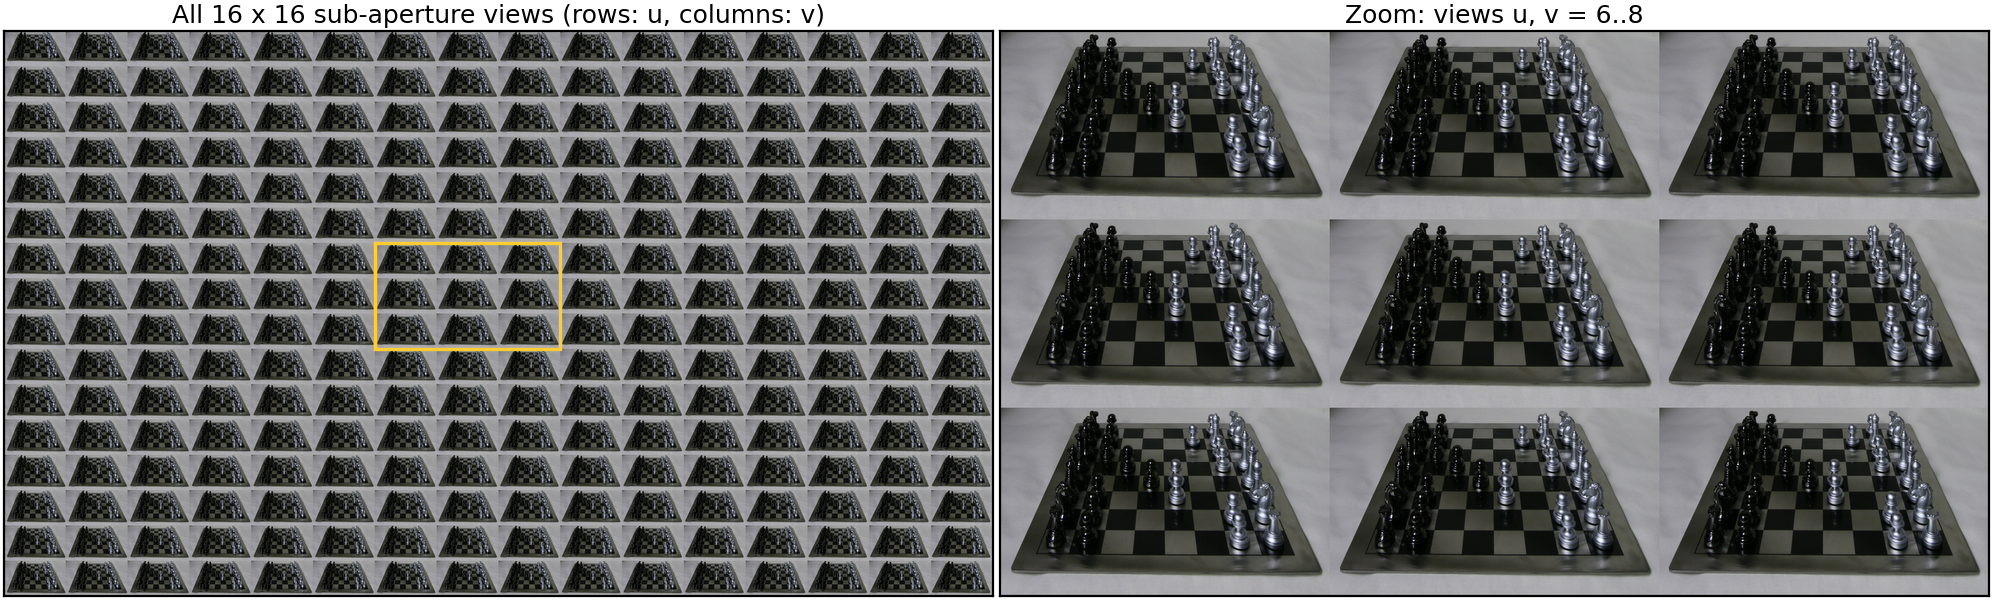
\includegraphics[width=\linewidth]{p1_mosaic.png}
\caption{Mosaic of the $16\times16$ sub-aperture views (rows: increasing $u$; columns: increasing $v$), and a zoom on the $3\times3$ views with $u,v$ indices 6--8, near the center of the aperture.}
\label{fig:p1mosaic}
\end{figure}

\subsection*{Refocusing and focal-stack simulation}
\begin{figure}[H]
\centering
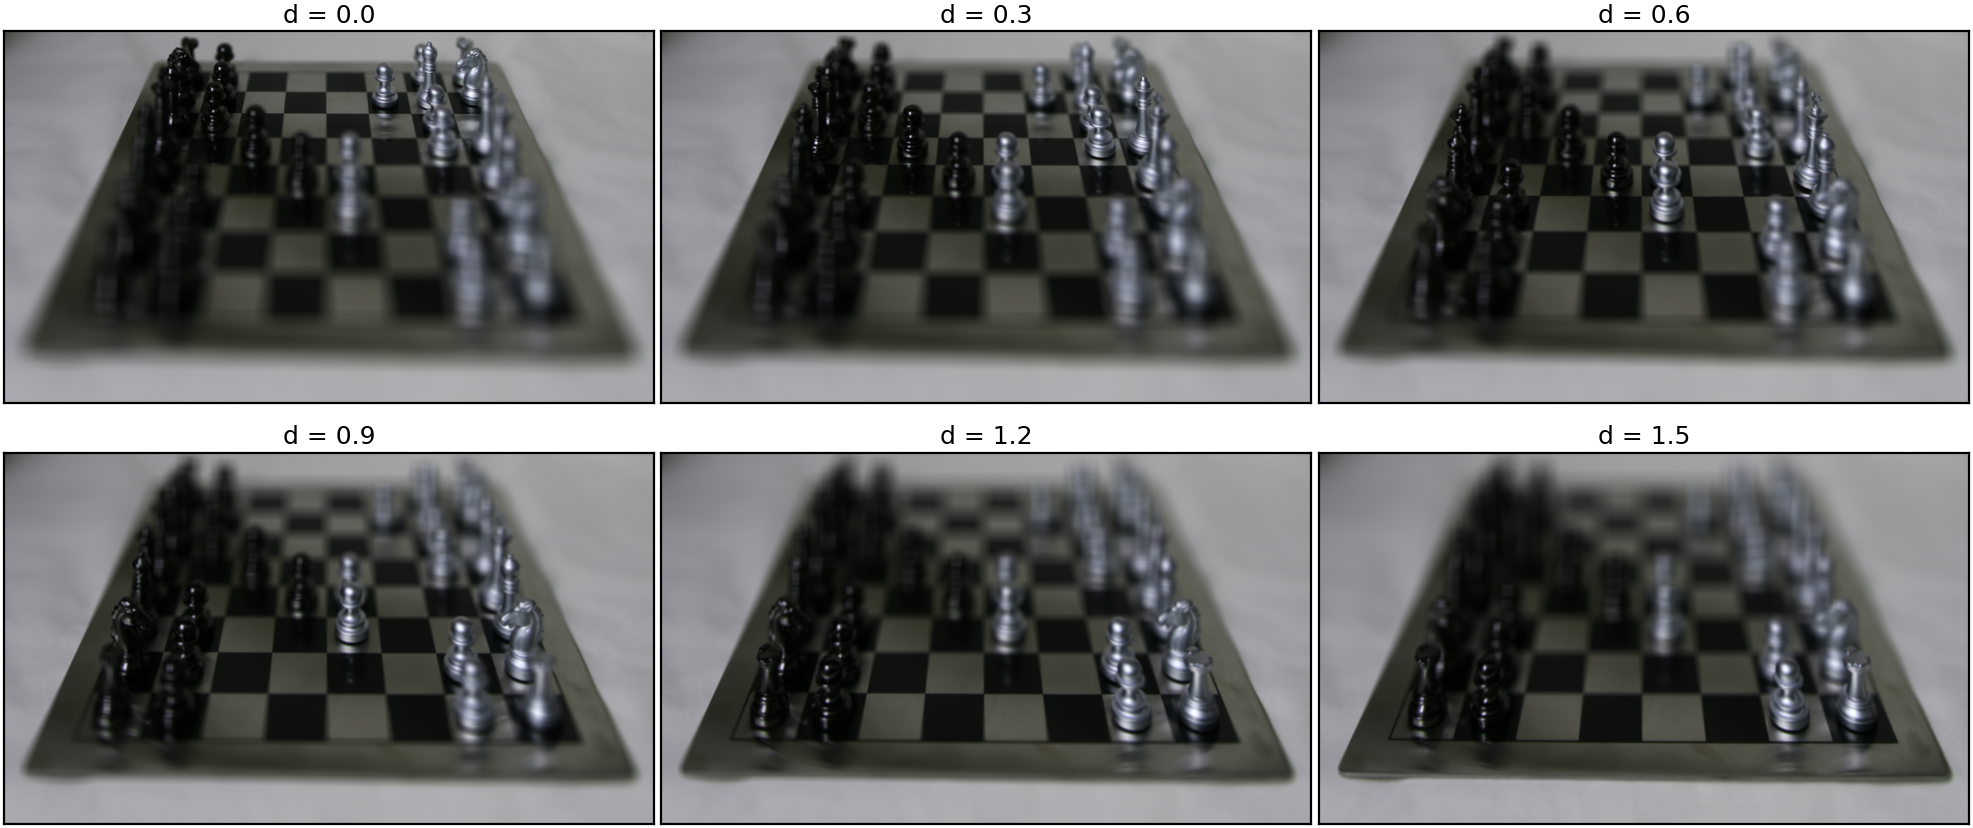
\includegraphics[width=\linewidth]{p1_refocus.png}
\caption{Refocusing with the largest aperture for six of the 16 values of $d$. As $d$ increases, the plane of focus moves from the back of the board to the front pieces.}
\label{fig:p1refocus}
\end{figure}

\subsection*{All-in-focus image and depth from focus}
\begin{figure}[H]
\centering
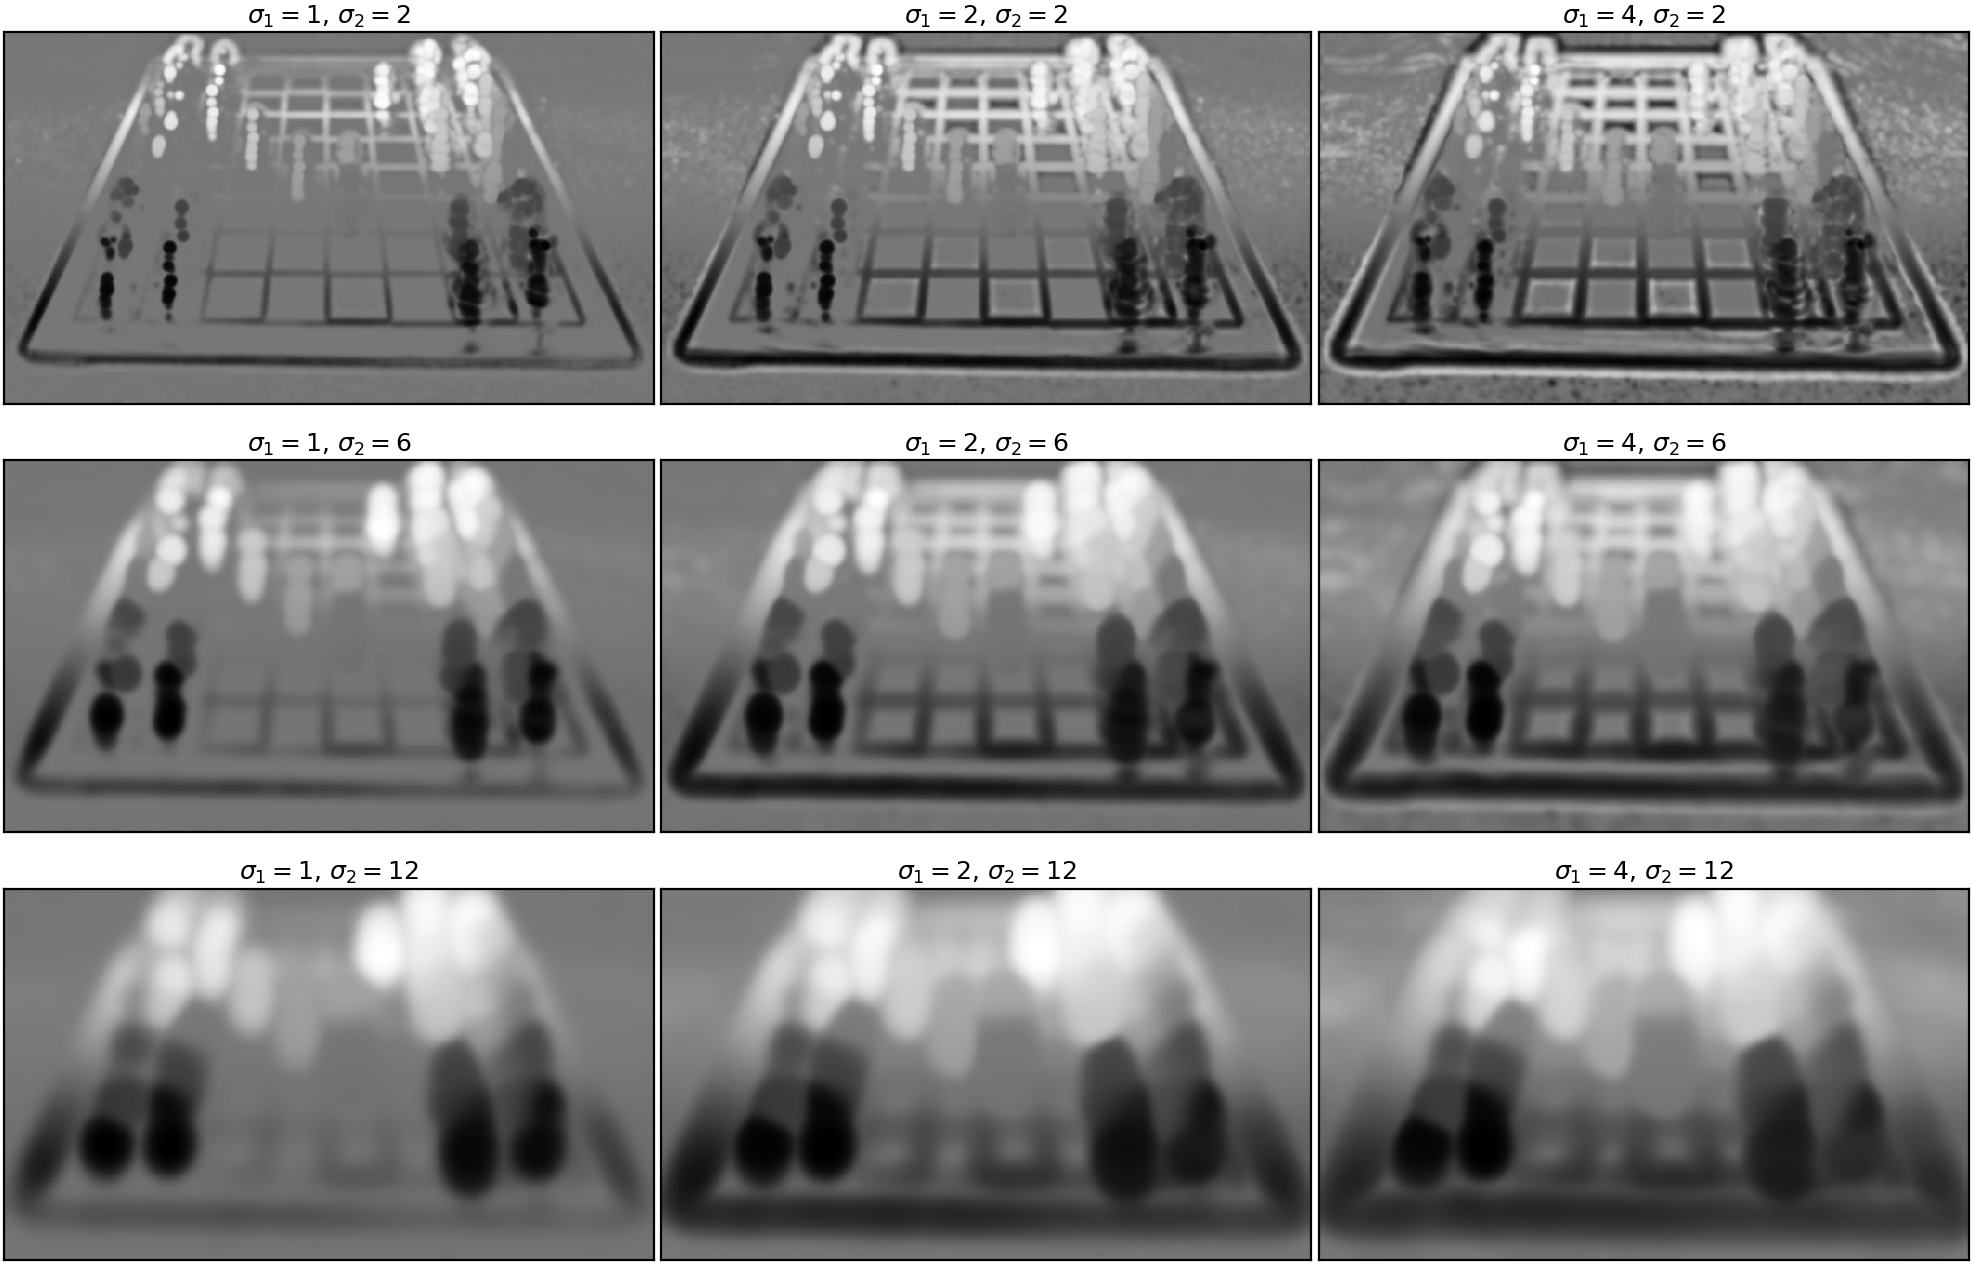
\includegraphics[width=0.92\linewidth]{p1_dff_sweep_depth.png}
\caption{Depth maps for $\sigma_1\in\{1,2,4\}$ (columns) and $\sigma_2\in\{2,6,12\}$ (rows). Brighter pixels are focused at smaller $d$.}
\label{fig:p1sweepdepth}
\end{figure}
\begin{figure}[H]
\centering
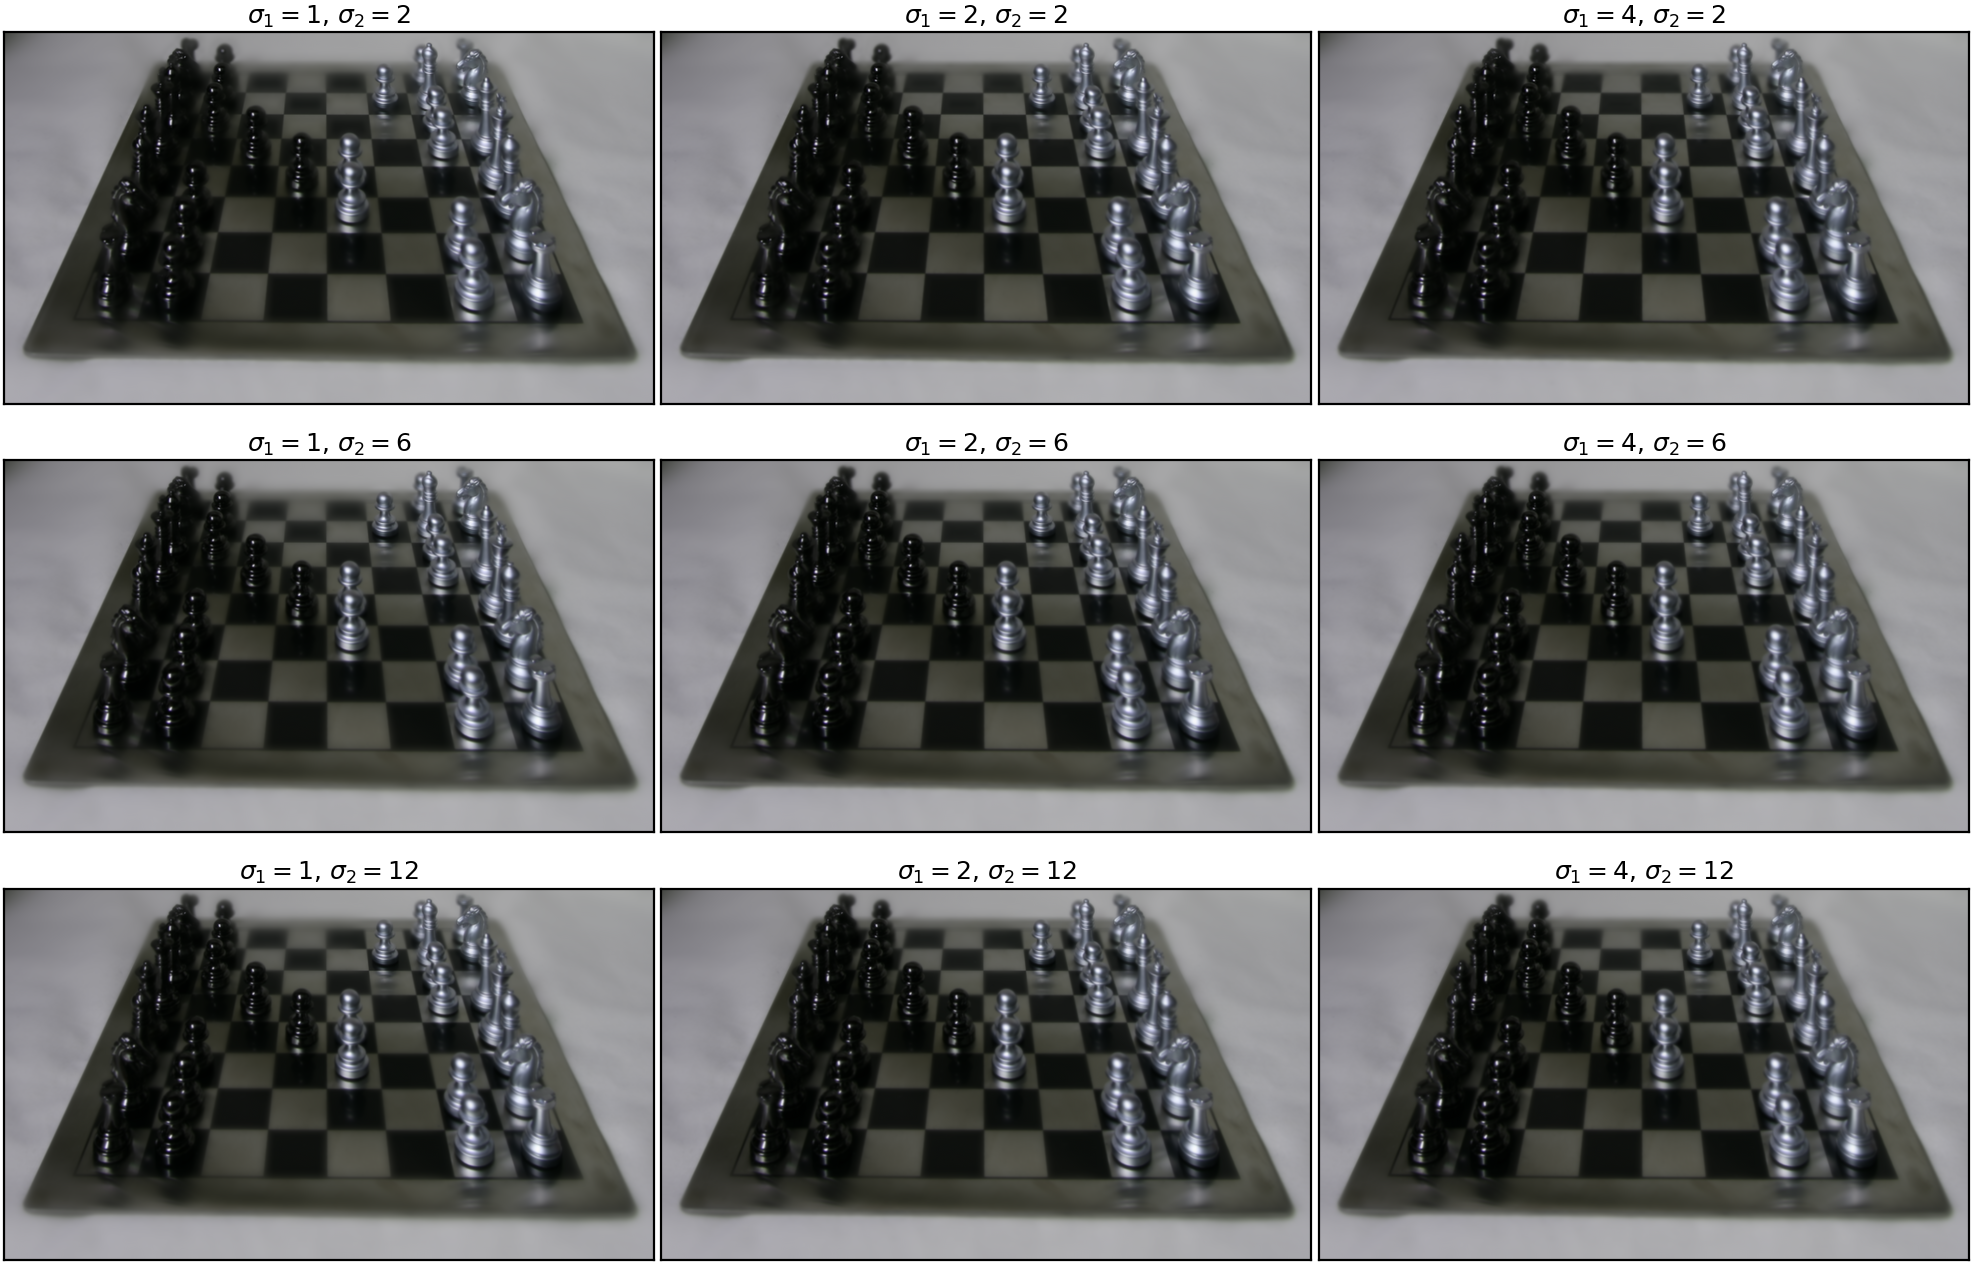
\includegraphics[width=0.92\linewidth]{p1_dff_sweep_aif.png}
\caption{All-in-focus images for the same grid of $\sigma_1$ and $\sigma_2$.}
\label{fig:p1sweepaif}
\end{figure}
\begin{figure}[H]
\centering
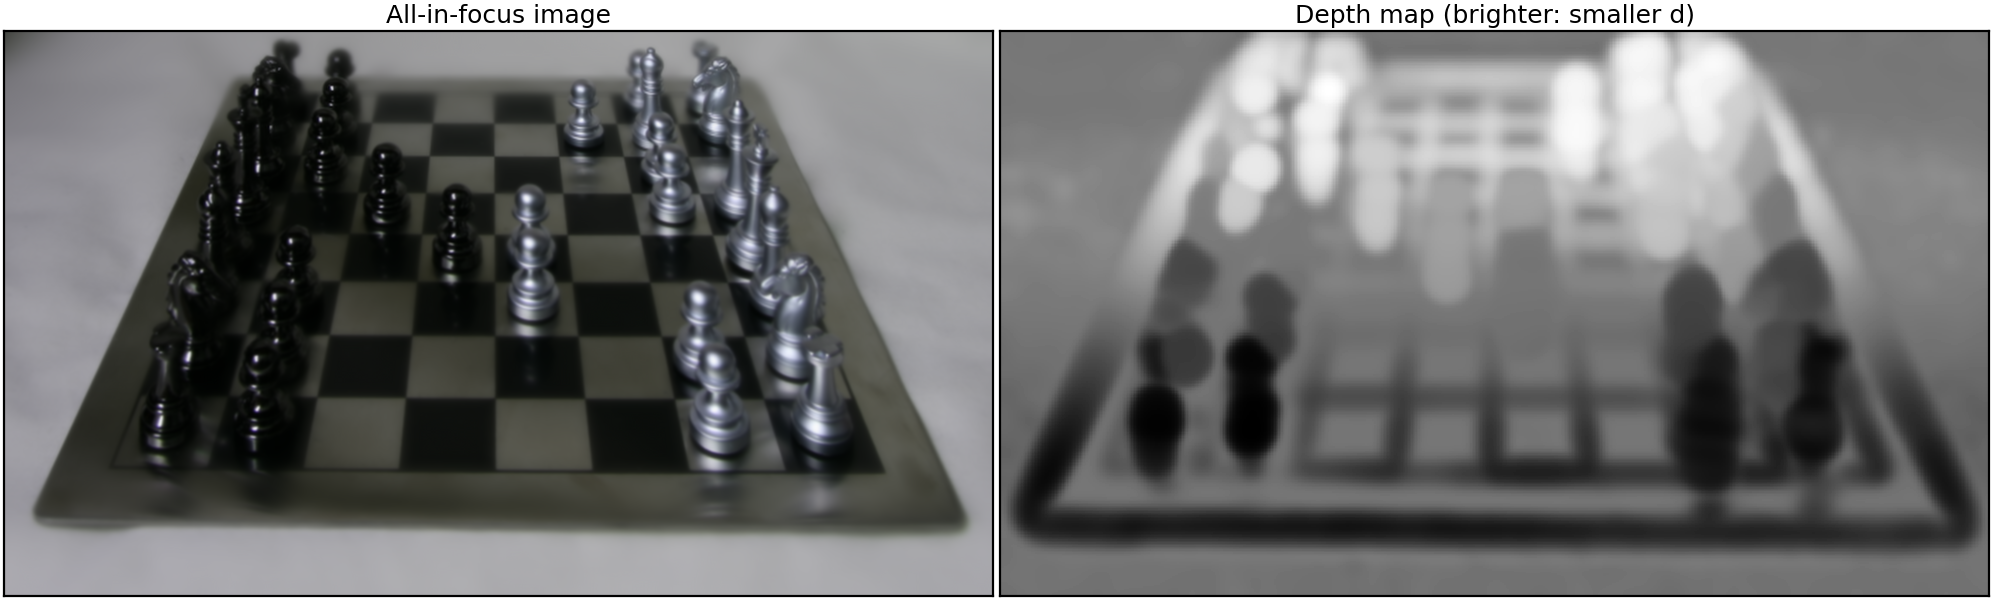
\includegraphics[width=\linewidth]{p1_dff_final.png}
\caption{All-in-focus image and depth map with the selected parameters ($\sigma_1=2$, $\sigma_2=6$).}
\label{fig:p1dff}
\end{figure}

\subsection*{Focal-aperture stack and confocal stereo}
\begin{figure}[H]
\centering
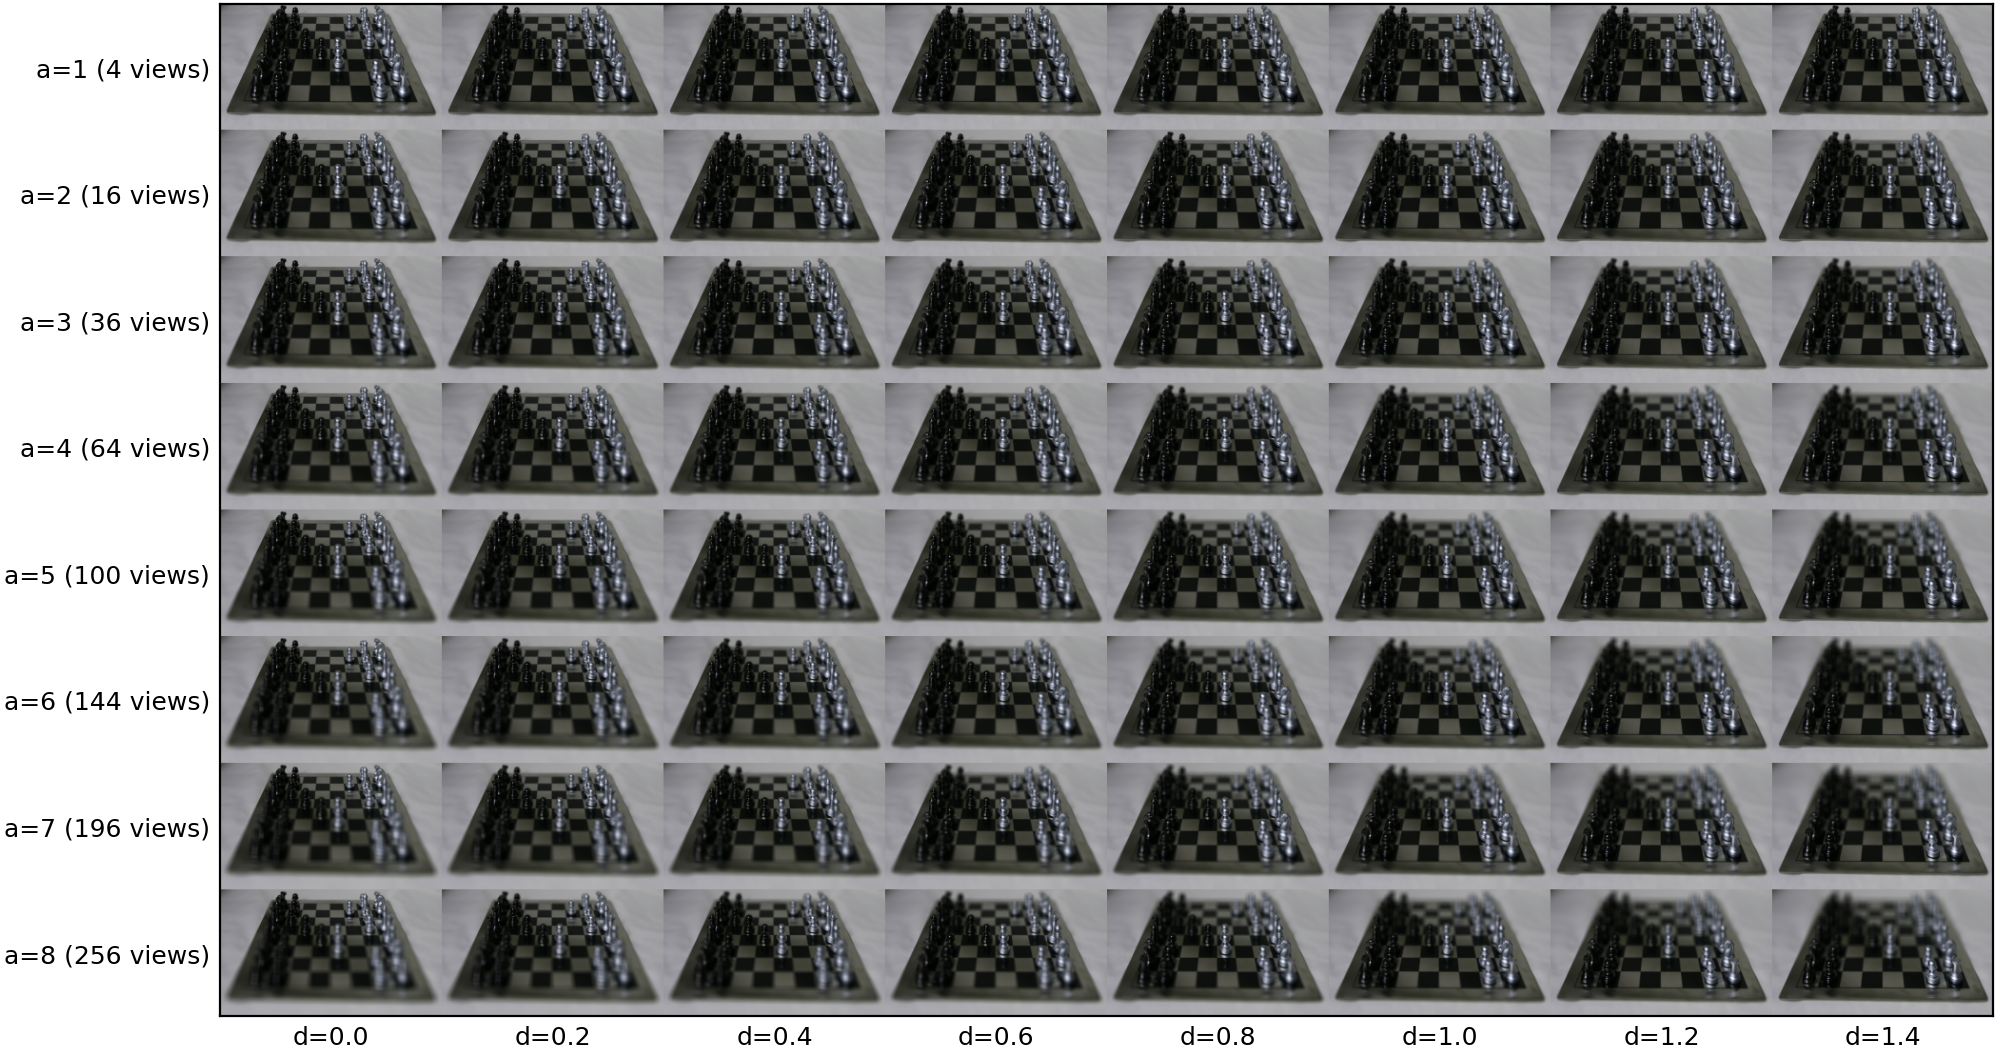
\includegraphics[width=\linewidth]{p1_af_collage.png}
\caption{Focal-aperture stack: square apertures $a=1,\dots,8$ (rows) and every other value of $d$ (columns; the stack uses all 16). Each image is divided by its number of views, so all apertures have the same exposure.}
\label{fig:p1afcollage}
\end{figure}
\begin{figure}[H]
\centering
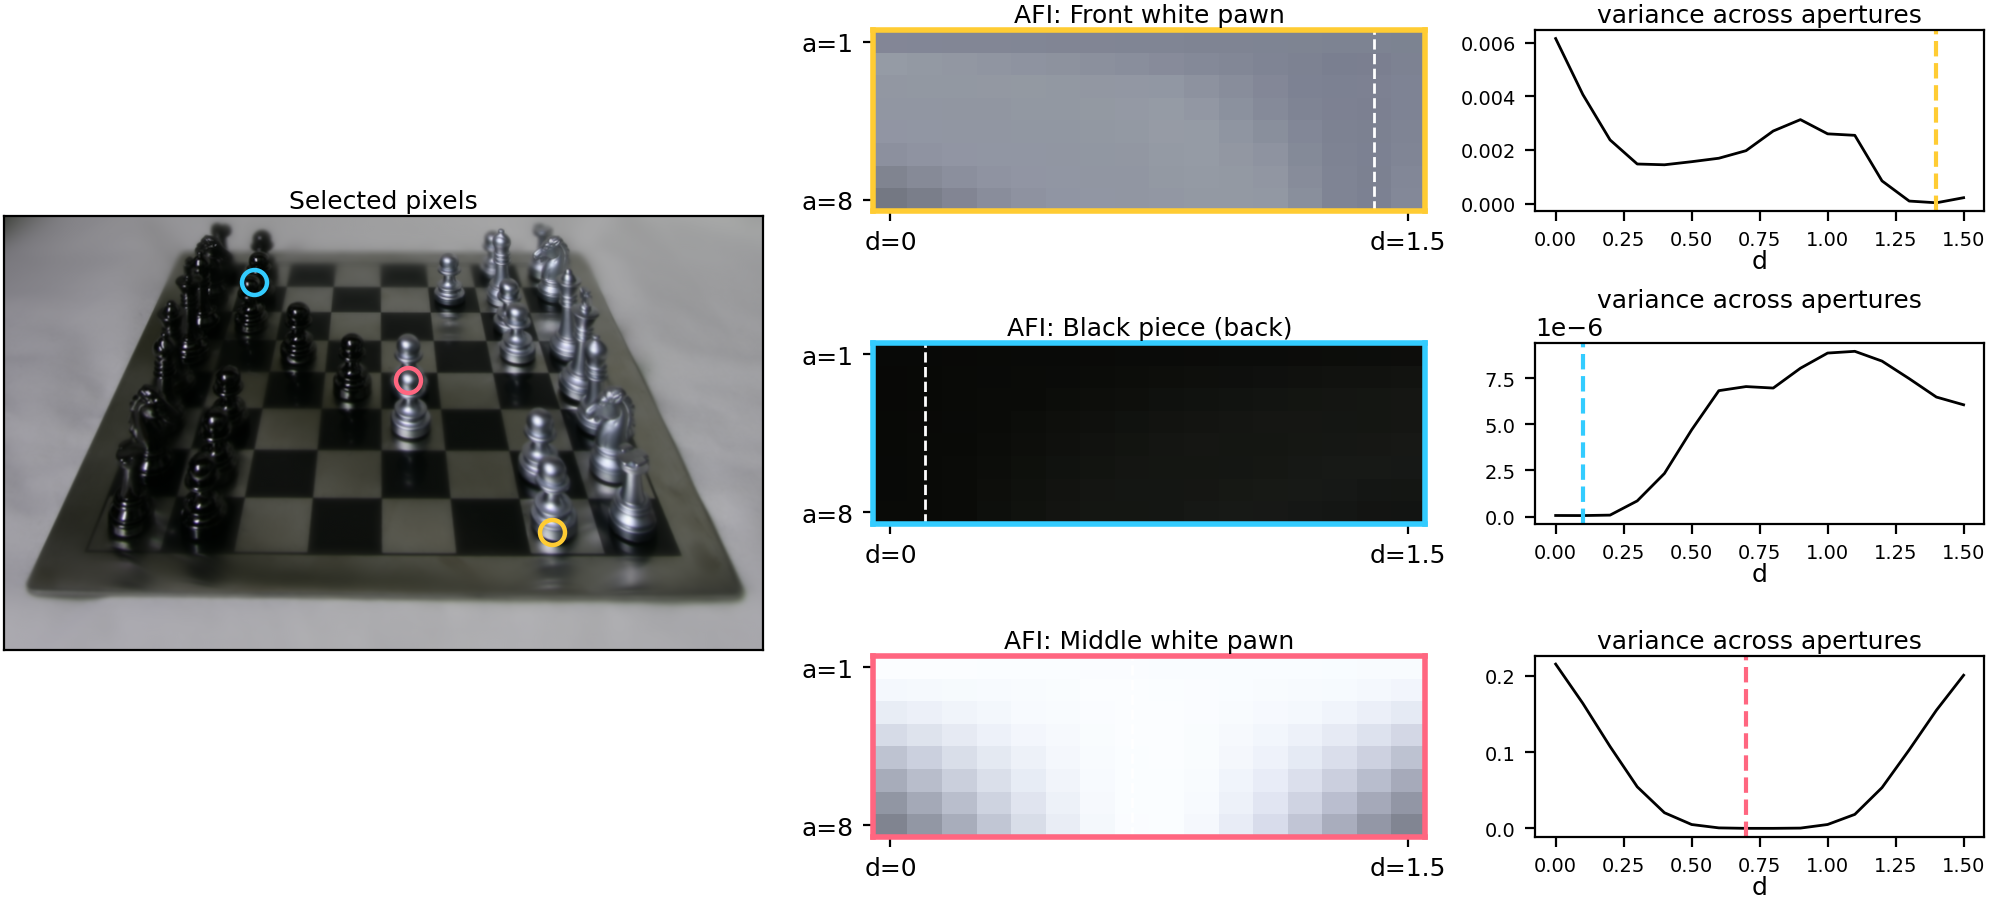
\includegraphics[width=\linewidth]{p1_afi.png}
\caption{Aperture-focus images (AFIs) at three pixels. Each AFI shows the color of the pixel for every aperture (rows) and every $d$ (columns); at the correct $d$ the colors agree across apertures (confocal constancy), and the variance across apertures (right) is smallest. The dashed lines mark the selected $d$.}
\label{fig:p1afi}
\end{figure}
\begin{figure}[H]
\centering
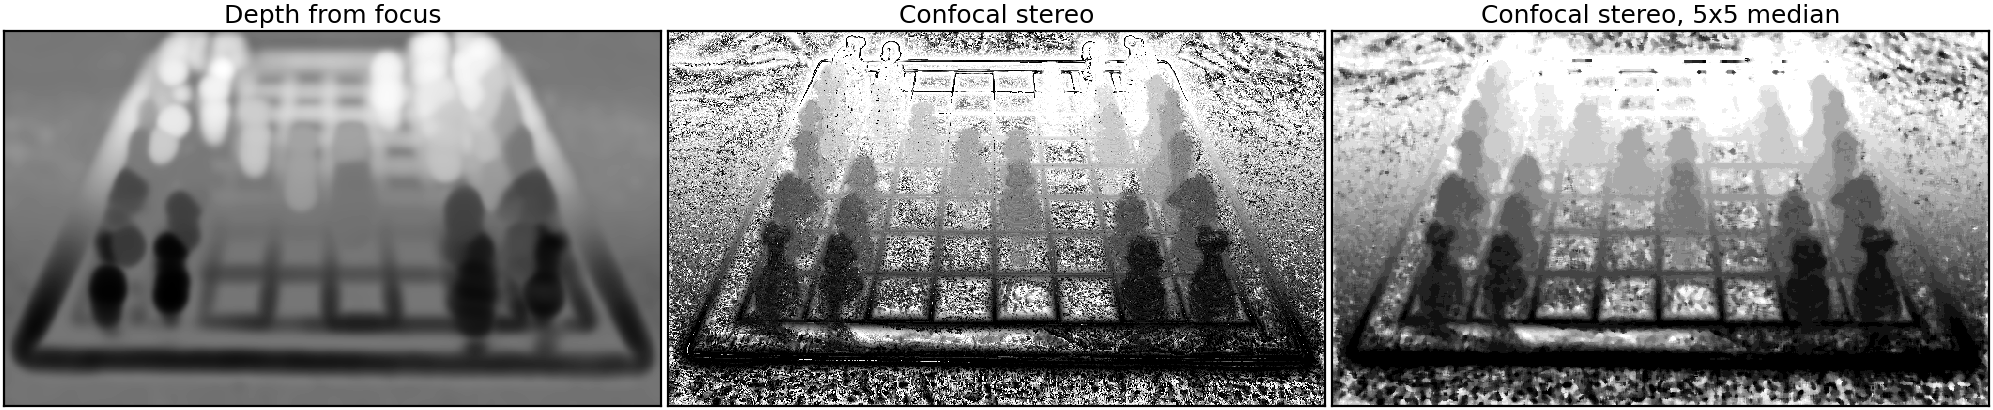
\includegraphics[width=\linewidth]{p1_confocal_vs_dff.png}
\caption{Depth from focus ($\sigma_1=2$, $\sigma_2=6$) and confocal stereo (per-pixel $\arg\min$, and after a $5\times5$ median filter for comparison). Brighter pixels are focused at smaller $d$.}
\label{fig:p1confocal}
\end{figure}

%======================================================================
\clearpage
\section{Bonus: Better blending and depth map}
%======================================================================
\subsection*{Method}
I adapted the blur-estimation and depth-fitting steps of Suwajanakorn et al., ``Depth from Focus with Your Mobile Phone'' (CVPR 2015), to the synthetic focal stack of Part~1. Instead of averaging the depth values with sharpness weights (Equation~(8)), this method models how much each image of the stack is blurred at every pixel and fits one depth per pixel that explains all of these blur measurements.
\begin{enumerate}\setlength{\itemsep}{2pt}
\item \textbf{All-in-focus reference.} For each pixel I keep the RGB value of the frame with the largest smoothed Laplacian-of-Gaussian response ($|\nabla^2 G_1 * Y|$ smoothed with $\sigma=2$). Unlike the weighted average of Equation~(7), this does not mix sharp and blurred frames.
\item \textbf{Blur estimation} (Equations~(7)--(9) of the paper). The all-in-focus image is blurred with PSFs of radius $r=0,0.25,\dots,r_{\max}$; for every frame $i$ and pixel, the cost is the mean absolute RGB difference between frame $i$ and the blurred reference, smoothed with a Gaussian of standard deviation $\sigma$. The blur radius $B_i$ is the radius with the smallest cost, and the confidence $C_i=(\bar c_i-\min_r c_i)^2$ measures how far the minimum dips below the average cost; it is low in textureless regions.
\item \textbf{Depth fitting} (Equation~(10) of the paper). I tried two blur models:
\begin{itemize}\setlength{\itemsep}{0pt}
\item \emph{Refocus model.} For a synthetic lightfield stack the refocus parameters $d_i$ are known and the blur is proportional to the distance in $d$: $B_i\approx k\,|d_i-d|$. I use a square PSF (the shape of the simulated aperture), $r_{\max}=12$ and $\sigma=2$. The scale $k$ is fitted on 800 sample pixels ($k=7.95$), and then the depth $d$ of every pixel is solved exactly: the cost $\sum_i C_i^2(k|d_i-d|-B_i)^2$ is piecewise quadratic in $d$, so I minimize it on every interval between consecutive $d_i$ and keep the best.
\item \emph{Thin-lens model.} This is the model of the paper, $B_i=A\,\frac{|f_i-s|}{s}\,\frac{F}{f_i-F}$, with unknown aperture $A$, focal length $F$ and focus distances $f_i$ (constrained to be ordered, with the first and last fixed at 10 and 32 arbitrary units), and a disk PSF with $r_{\max}=16$ and $\sigma=3$. The global parameters are fitted with sparse nonlinear least squares on a sample of pixels, and the per-pixel depths are then solved as above in inverse depth.
\end{itemize}
\end{enumerate}
Both models fit the blur measurements to a confidence-weighted RMS error of about 0.41\,px (Table~\ref{tab:b2params}). Compared with the paper, I omit the MRF-based all-in-focus stitching, the bokeh correction and the final spatial refinement of the depth map.

\subsection*{Discussion}
\begin{itemize}\setlength{\itemsep}{2pt}
\item \textbf{Comparison with Part 1.} Instead of averaging depth values with sharpness weights, this method estimates how much each frame is blurred at every pixel and fits a lens model (the thin-lens model, or the simpler refocus model) to these blur measurements. Compared with Part 1, the resulting depth maps contain much more detail, with clear outlines of the individual chess pieces, and they largely avoid the dot-like errors of the confocal-stereo depth map (Figures~\ref{fig:b2compare} and~\ref{fig:b2zoom}).
\item \textbf{Missing refinement.} I did not implement the refinement step of the paper, which uses the confidence of the blur estimates to refine the depth map. As a result, regions with low confidence, such as the textureless background and the interiors of some board squares, still contain noisy depth values.
\end{itemize}

\begin{table}[!htbp]
\centering
\small
\begin{tabular}{llll}
\toprule
Model & PSF & Blur estimation & Fit \\
\midrule
Refocus & square, $r\le12$ & $\sigma=2$ & $k=7.95$; weighted RMS 0.42\,px; 4.6\,s \\
Thin lens & disk, $r\le16$ & $\sigma=3$ & $A=567$, $F=0.35$; weighted RMS 0.41\,px; 10.4\,s \\
\bottomrule
\end{tabular}
\caption{Parameters and fit statistics of the two blur models (full $400\times700$ resolution).}
\label{tab:b2params}
\end{table}

\clearpage
\subsection*{Results}
\begin{figure}[H]
\centering
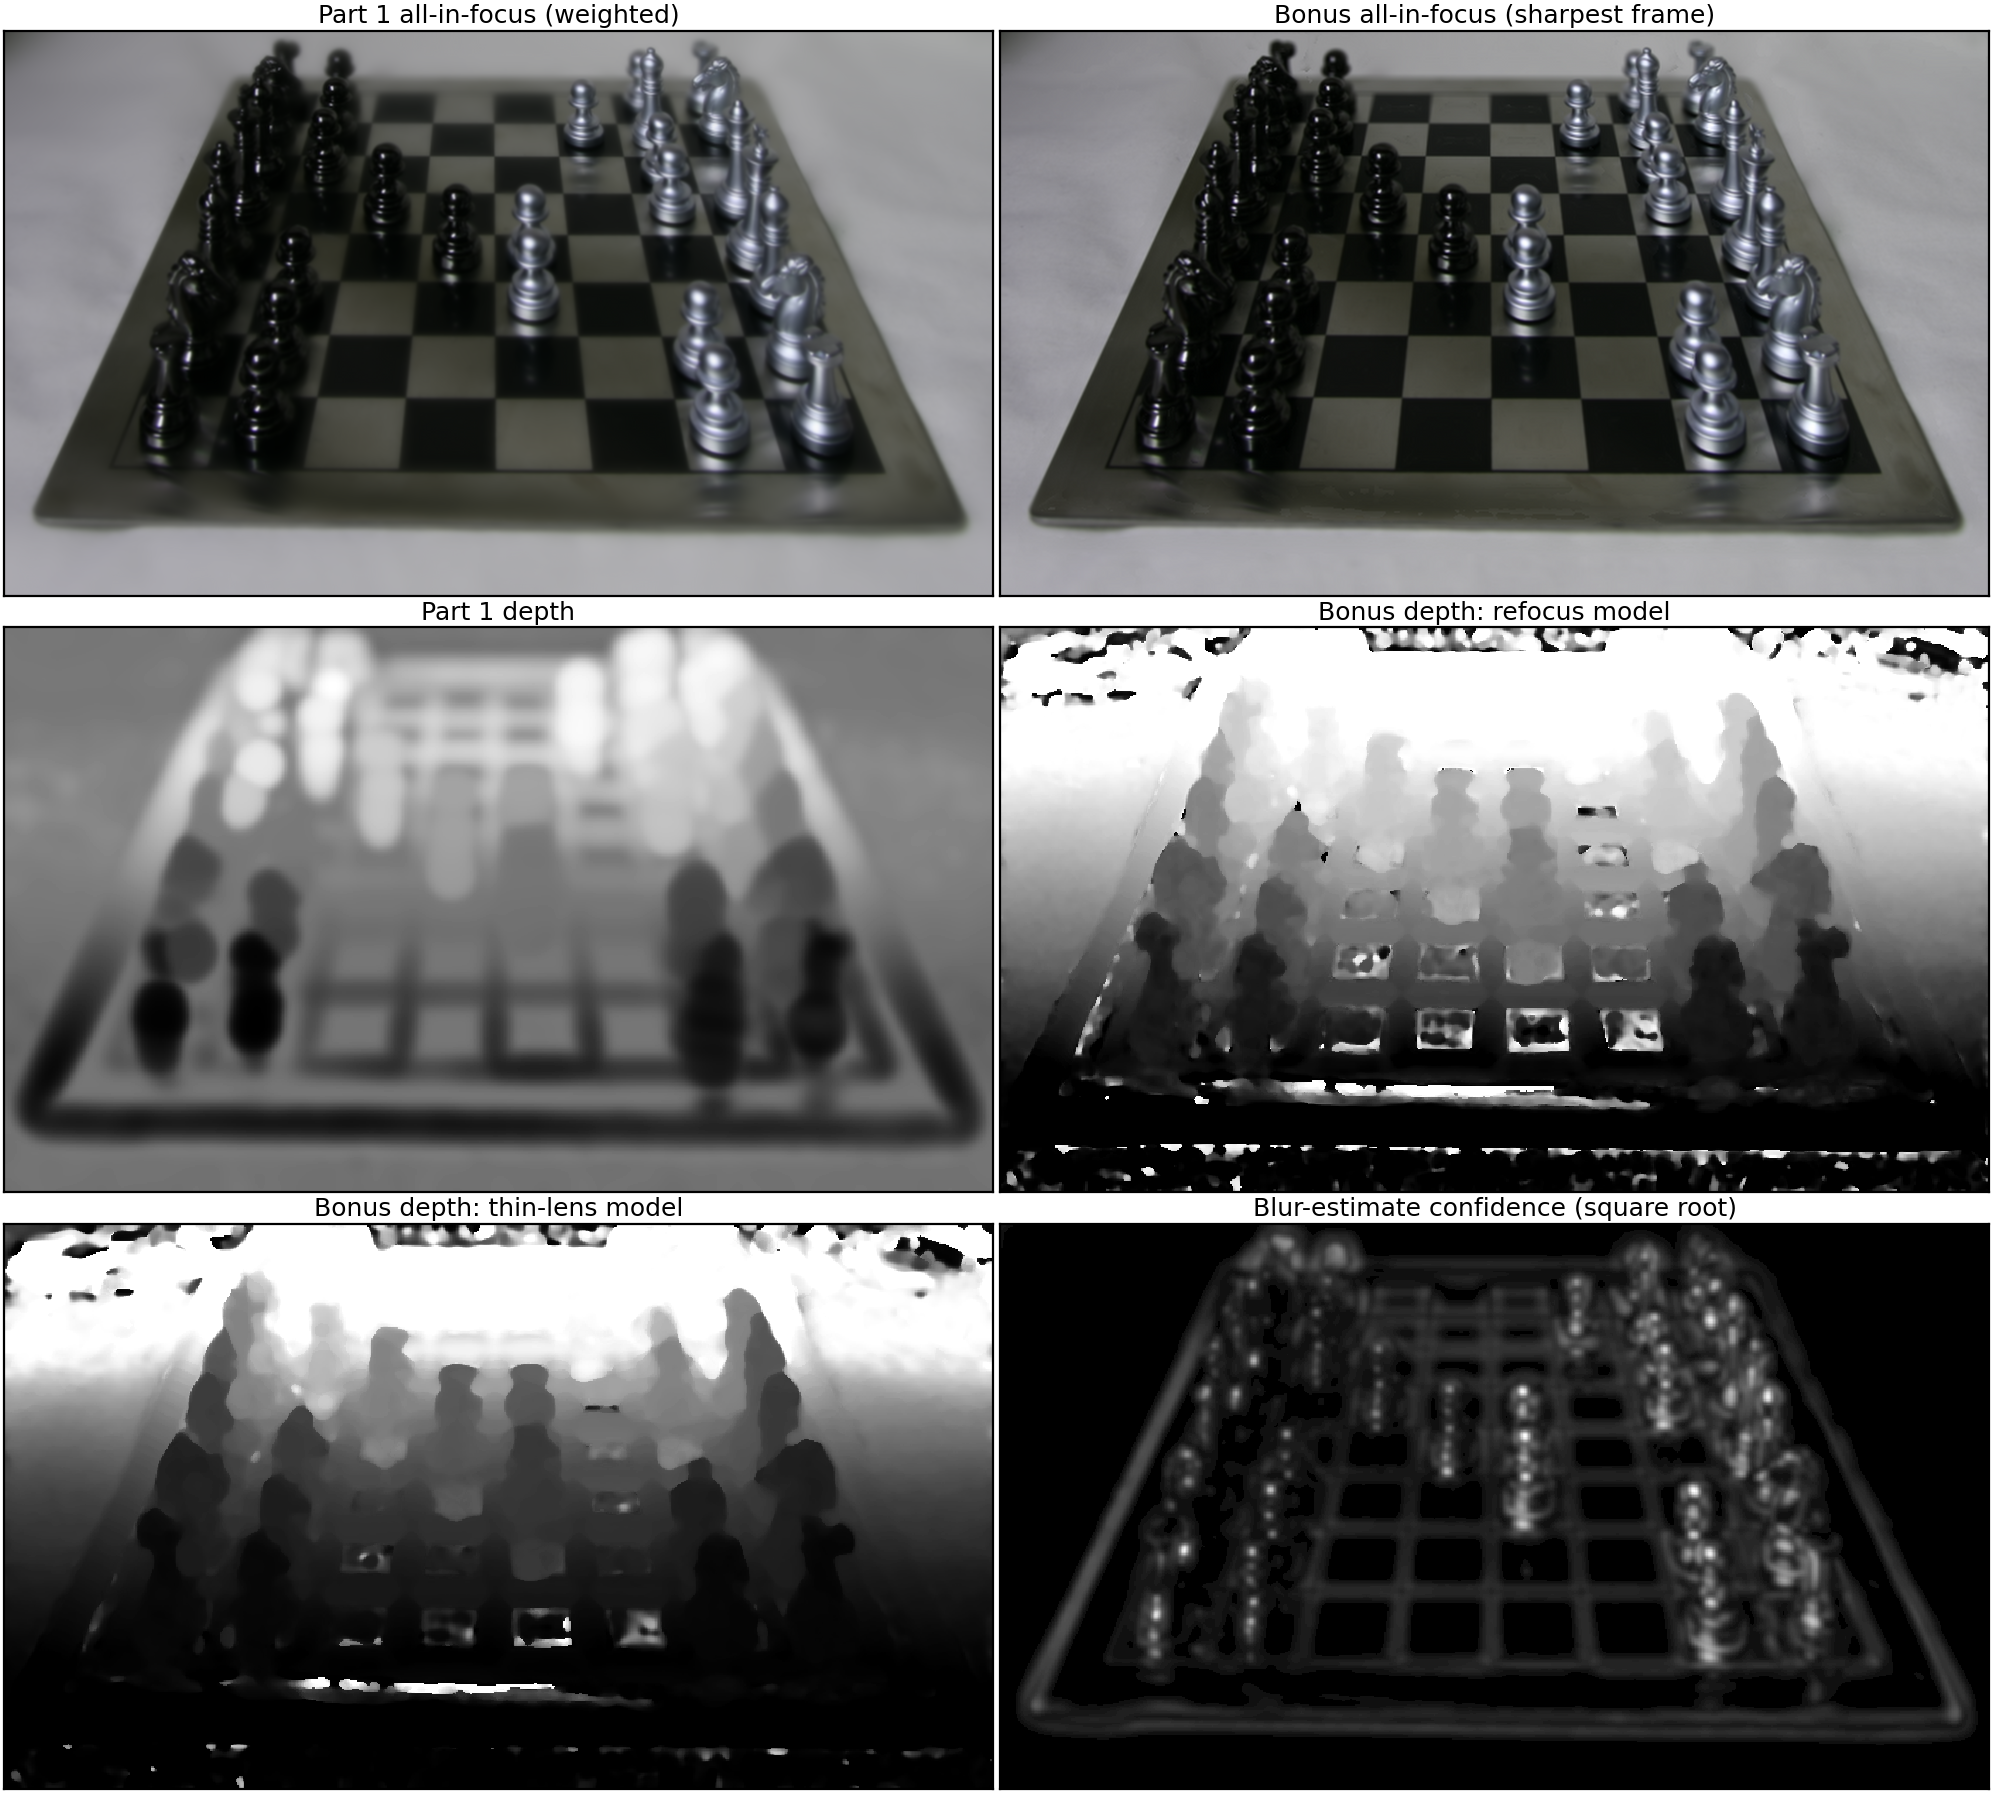
\includegraphics[width=\linewidth]{b2_compare.png}
\caption{Top: all-in-focus images of Part~1 (weighted average, Equation~(7)) and of the bonus pipeline (sharpest frame per pixel). Middle: depth maps of Part~1 and of the refocus model. Bottom: depth map of the thin-lens model and the blur-estimate confidence (summed over frames, shown as its square root). Brighter pixels are focused at smaller $d$.}
\label{fig:b2compare}
\end{figure}
\begin{figure}[H]
\centering
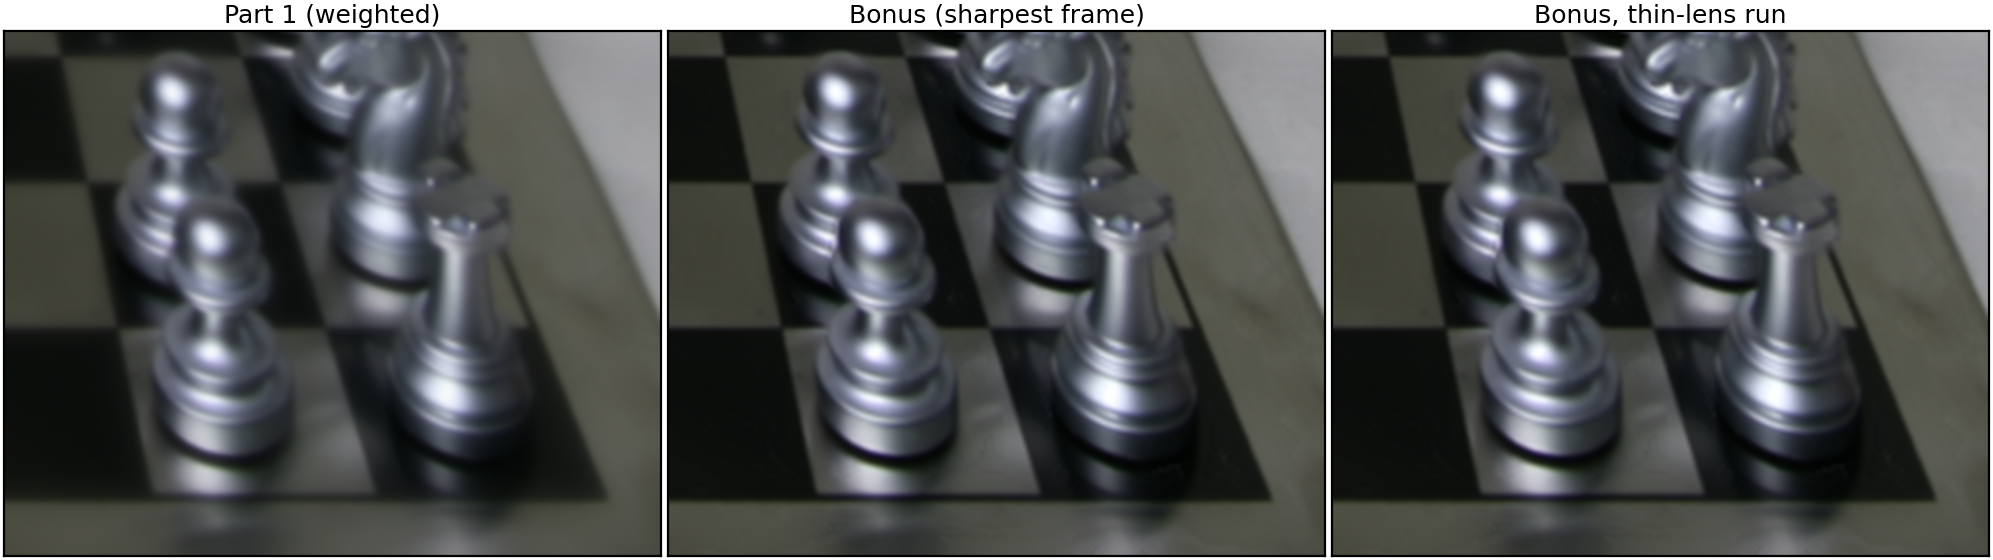
\includegraphics[width=\linewidth]{b2_zoom.png}
\caption{Zoom on the front pieces in the all-in-focus images.}
\label{fig:b2zoom}
\end{figure}

%======================================================================
\clearpage
\section{Capture and refocus your own lightfield}
%======================================================================
\subsection*{Capture}
I recorded a 4.2\,s video (126 frames, $1080\times1920$, 30\,fps) with my phone while moving it in a plane, in a zig-zag pattern, in front of three figures placed at different depths on a desk (Figure~\ref{fig:p3frames}). Focus, exposure and zoom were kept fixed during the recording.

\subsection*{Implementation}
\begin{itemize}\setlength{\itemsep}{2pt}
\item \textbf{Preprocessing.} Every frame is converted to linear RGB in $[0,1]$, and template matching uses its luminance $Y$ (XYZ).
\item \textbf{Normalized cross-correlation with correlations only.} Let $\tilde g=g-\bar g$ be the zero-mean template with $n$ pixels and $\mathbf 1$ an all-ones kernel of the template size. Because $\sum\tilde g=0$, the term $\bar I_t$ in the numerator of Equation~(9) vanishes, and the denominator follows from $\sum(I-\bar I)^2=\sum I^2-(\sum I)^2/n$:
\begin{equation*}
h_t=\frac{I_t\star\tilde g}{\sqrt{\big(\sum\tilde g^2\big)\big(I_t^2\star\mathbf 1-(I_t\star\mathbf 1)^2/n\big)}},
\end{equation*}
where $\star$ is \texttt{scipy.signal.correlate2d} with \texttt{mode='valid'}, so that $h_t[i,j]$ is the score of the template with its top-left corner at $(i,j)$. These are three correlations and pixel-wise operations; a small constant in the denominator avoids division by zero in flat regions. I verified that the result matches OpenCV's \texttt{TM\_CCOEFF\_NORMED}.
\item \textbf{Search window.} The template is selected in the first frame. Instead of one large window centered on the template, each frame is searched only within $\pm30$ pixels of the match in the previous frame, because the camera moves little between consecutive frames but the total shift over the video is more than 140\ pixels. This keeps the correlations small and avoids false matches on similar structures elsewhere in the frame (Figure~\ref{fig:p3ncc}).
\item \textbf{Shift and merge.} With $[s_{t,y},s_{t,x}]$ the position of the match relative to frame 0, every frame is shifted by $-[s_{t,y},s_{t,x}]$ with integer shifts, so that the template lands at the same position in all frames. Pixels shifted in from outside the frame are zero-padded and excluded from the average: the sum of the shifted frames is divided per pixel by the number of frames that cover it. The result is gamma-encoded for display.
\end{itemize}

\subsection*{Discussion}
\begin{itemize}\setlength{\itemsep}{2pt}
\item \textbf{Refocusing.} Template matching successfully refocuses the video at the depths of all three figures: in each result the selected figure is sharp, while the figures at other depths are blurred (Figures~\ref{fig:p3refocus} and~\ref{fig:p3zoom}).
\item \textbf{Ghosting.} The out-of-focus figures show ghosting artifacts: instead of a smooth blur, they appear as several overlapping copies. This is likely caused by the uneven speed of the camera motion during capture. Each frame corresponds to one sample on the aperture plane, so where I moved the camera slowly, many frames sample nearly the same position, while fast motion leaves gaps between the samples (Figure~\ref{fig:p3shifts}). The synthetic aperture is therefore sampled unevenly, and the sum of the shifted frames contains a few distinct copies instead of a uniform blur.
\end{itemize}

\begin{table}[!htbp]
\centering
\small
\begin{tabular}{ll}
\toprule
Step & Parameters \\
\midrule
Video & 126 frames, $1080\times1920$, 30\,fps; all frames used \\
Templates & $145\times140$ (near), $175\times160$ (middle) and $120\times120$ (back) pixels ($w\times h$), selected in frame 0 \\
Search & $\pm30$ pixels around the previous match \\
Merge & integer shifts, zero padding, per-pixel count normalization \\
\bottomrule
\end{tabular}
\caption{Parameters for refocusing the unstructured lightfield.}
\label{tab:p3params}
\end{table}

\clearpage
\subsection*{Results}
\begin{figure}[H]
\centering
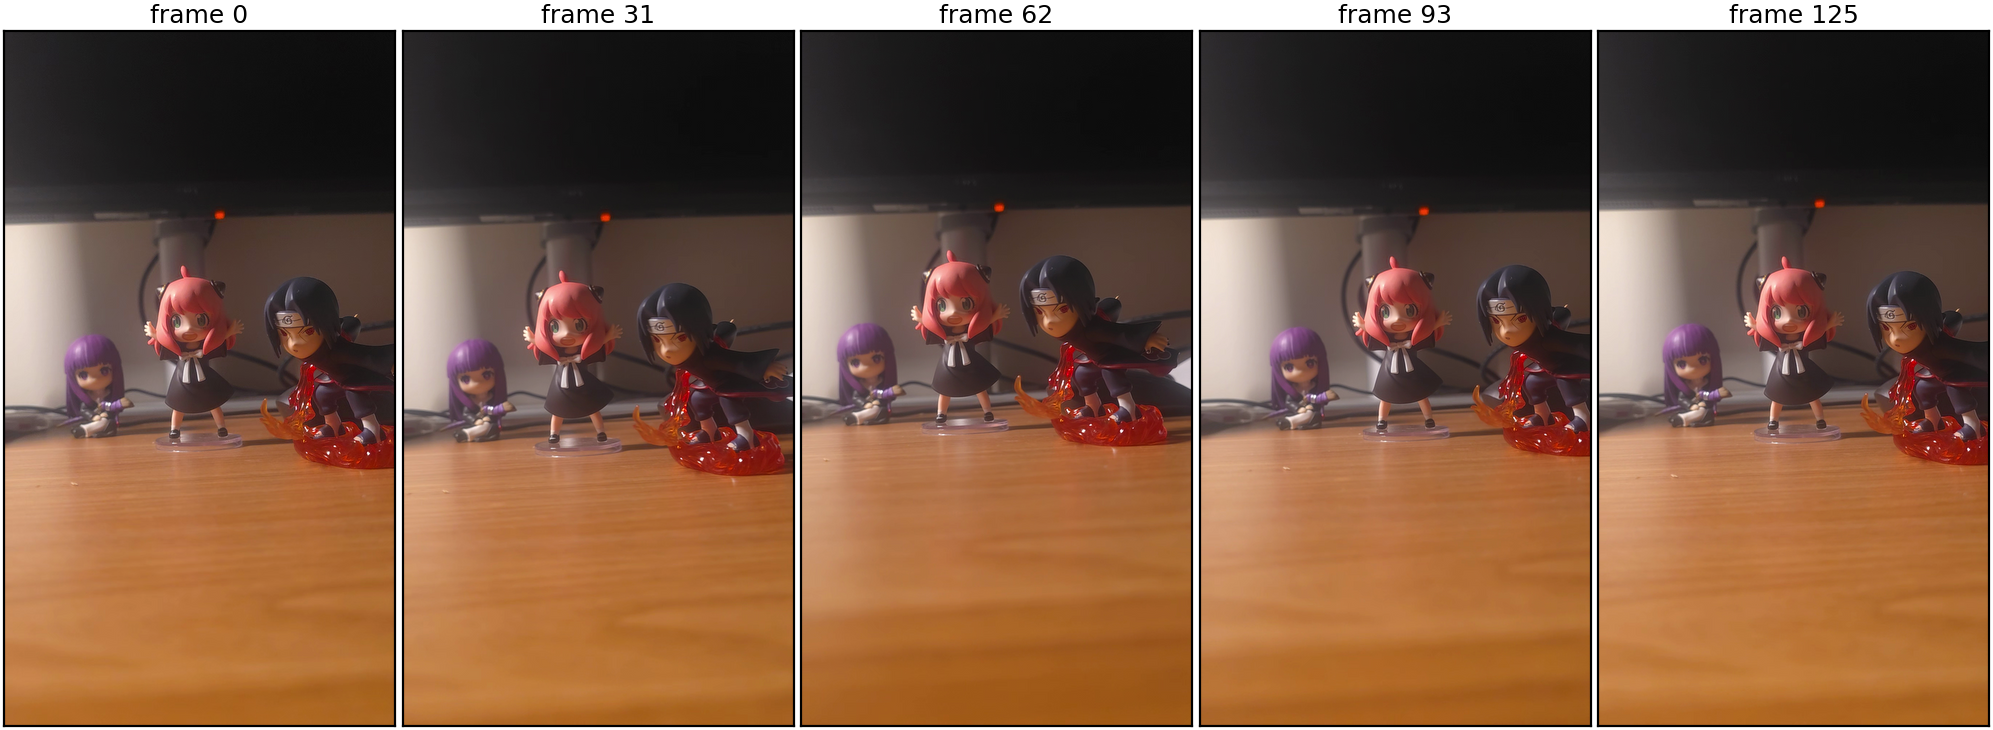
\includegraphics[width=\linewidth]{p3_frames.png}
\caption{Frames of the captured video.}
\label{fig:p3frames}
\end{figure}
\begin{figure}[H]
\centering
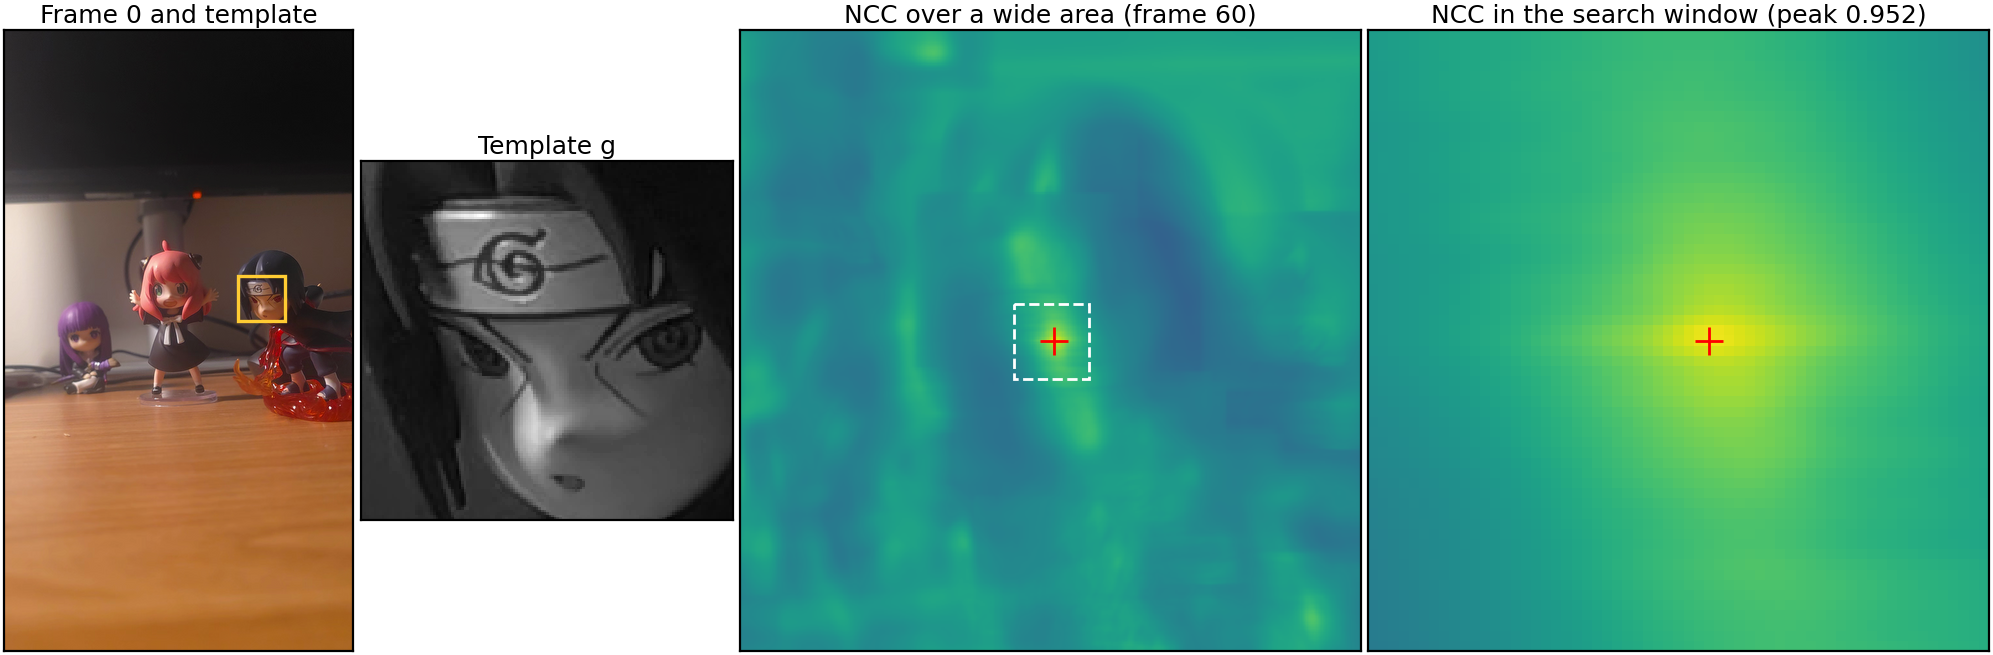
\includegraphics[width=\linewidth]{p3_ncc.png}
\caption{Template matching for the near figure. From left: frame 0 with the template, the template, the NCC map of frame 60\ over a large neighborhood (dashed: the search window used; red cross: selected match), and the NCC map inside the search window.}
\label{fig:p3ncc}
\end{figure}
\begin{figure}[H]
\centering
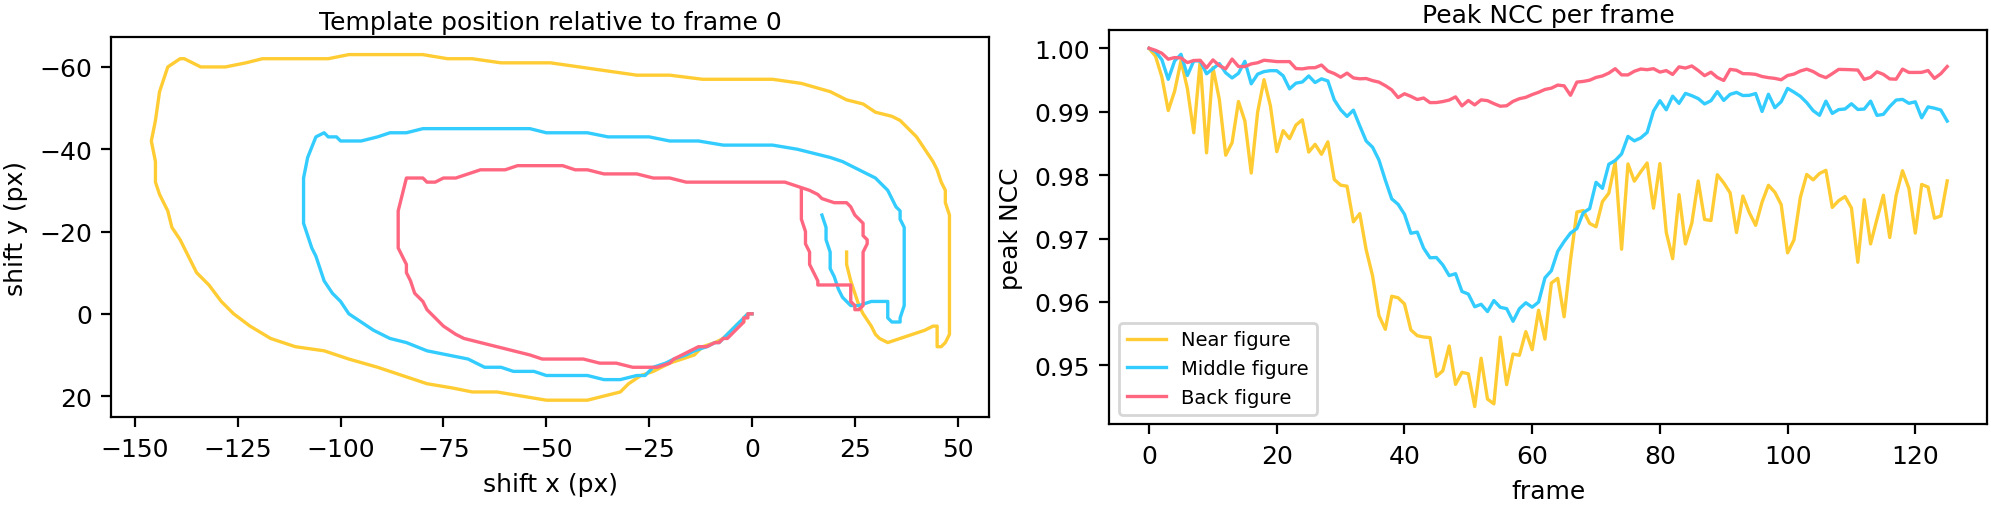
\includegraphics[width=\linewidth]{p3_shifts.png}
\caption{Left: position of each template in every frame relative to frame 0, which traces the camera path on the aperture plane. Right: peak NCC per frame.}
\label{fig:p3shifts}
\end{figure}
\begin{figure}[H]
\centering
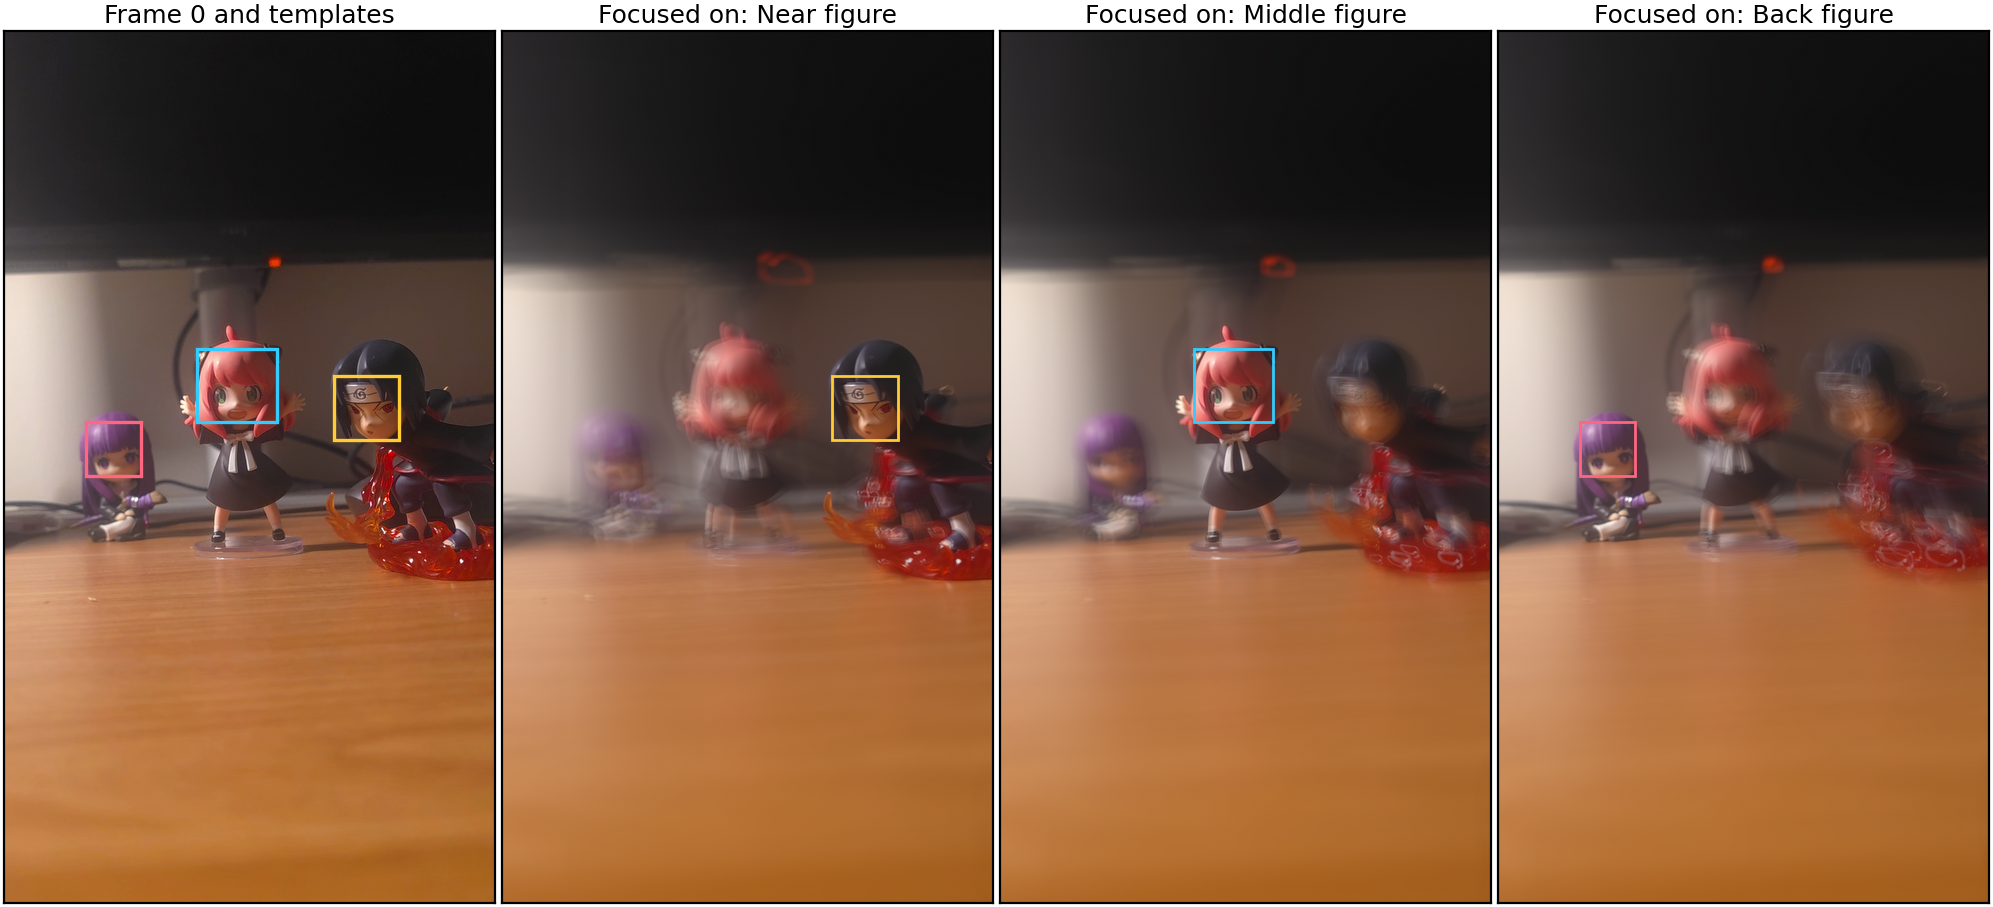
\includegraphics[width=\linewidth]{p3_refocus.png}
\caption{Refocusing on the three templates (boxes in frame 0).}
\label{fig:p3refocus}
\end{figure}
\begin{figure}[H]
\centering
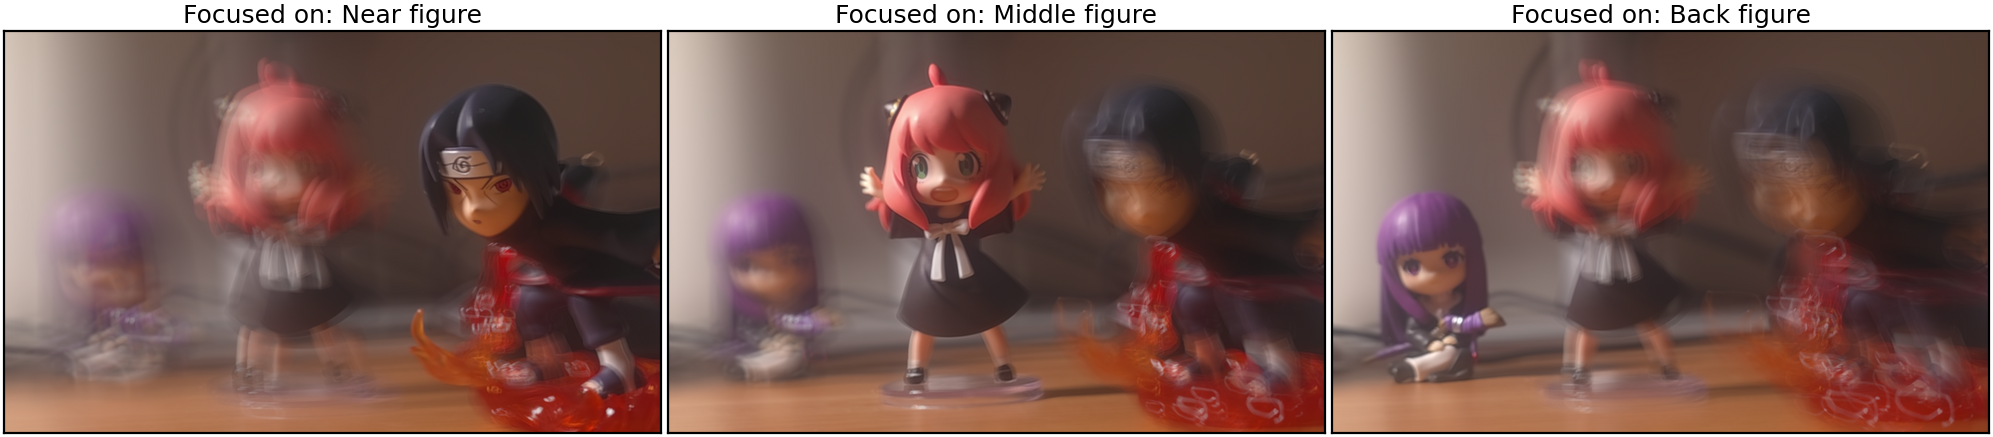
\includegraphics[width=\linewidth]{p3_refocus_zoom.png}
\caption{Zoom on the three figures in each refocused image.}
\label{fig:p3zoom}
\end{figure}

%======================================================================
\clearpage
\section{Bonus: Capture and process your own focal-aperture stack}
%======================================================================
\subsection*{Capture}
The stack was captured with a Nikon D3500 and the AF-P DX 18--55\,mm lens at 24\,mm, on a tripod and tethered to my laptop. I controlled the camera with \texttt{gphoto2} from a shell script (\texttt{capture\_stack.sh}), with the camera in manual exposure mode and the focus mode set to AF-S. For every aperture, the script first drives the focus to the far end of its range (\texttt{manualfocusdrive=1000}, repeated three times), then alternates \texttt{capture-image-and-download} and a focus step towards the near end. The capture settings were:
\begin{itemize}\setlength{\itemsep}{0pt}
\item 4 apertures: $f/4$, $f/5.6$, $f/8$ and $f/11$;
\item 8 focus settings, with focusing distances (from the EXIF data) of 8.41, 8.41, 0.89, 0.50, 0.38, 0.32, 0.25 and 0.25\,m;
\item 1/60\,s and ISO 400 for all images, saved as RAW (NEF).
\end{itemize}
To choose the focus steps, I first ran a coarse sweep at $f/4$ and checked, with a sharpness measure on a $3\times3$ grid of image regions, in which shots each part of the scene was sharpest. The scene is a desk with three figures at different depths, a mug and a monitor (Figure~\ref{fig:p4stack}). The NEF files are decoded with \texttt{dcraw -4 -T -w -h -o 1} into linear 16-bit images (half resolution, camera white balance, sRGB primaries), and downsampled to $1504\times1004$ pixels.

\subsection*{Alignment}
Changing the focus changes the magnification. I estimate one global similarity transform (scale, rotation and translation) per focus setting from the $f/11$ images, which have the largest depth of field: ORB features are matched between consecutive focus settings, the transform is fitted with RANSAC (\texttt{cv2.estimateAffinePartial2D}), and the transforms are chained back to the far-focus frame F0. The same transform is applied to all four apertures at that focus setting, and 3\% is cropped on every side.

The measured scale increases smoothly from 1.000 (F0) to 1.053 (F7), i.e., the near-focus images are about 5\% wider than the far-focus ones. The Gaussian lens formula predicts the opposite: with $f=24$\,mm, the image distance $s_i=(1/f-1/s_o)^{-1}$ is larger for near focus, so near-focus images should be about 10\% \emph{more} magnified. The reason is that this lens focuses internally (it moves a lens group instead of the whole lens), so its focal length changes with focus (``focus breathing'') and the single thin-lens model does not apply. I therefore use the measured transforms instead of the lens formula (Figure~\ref{fig:p4align}).

\subsection*{Processing}
\begin{itemize}\setlength{\itemsep}{2pt}
\item \textbf{Exposure equalization.} The measured brightness ratios between apertures do not follow $N^2$: relative to $f/4$, the $f/5.6$, $f/8$ and $f/11$ images have about 0.78, 0.42 and 0.26 of the brightness, instead of 0.51, 0.25 and 0.13. The ratios also change between focus settings (for example 0.30 instead of 0.25 at $f/11$ for F2 and F3), because daylight from a window changed during the capture. I therefore divide every image by a smooth gain map (ratio of Gaussian-blurred images, $\sigma=40$\,px, per channel) relative to the $f/4$ image at the same focus setting, which also removes the difference in vignetting between apertures. The whole stack is then scaled so that the median of the $f/4$ images is 0.18.
\item \textbf{Depth from focus and all-in-focus image.} The $f/4$ images (the shallowest depth of field) are merged with the pipeline of Part~1 on linear images, with $\sigma_1=2$ and $\sigma_2=10$.
\item \textbf{Confocal stereo.} As in Part~1, the cost is the variance of the linear intensities across the four apertures, summed over RGB, and the depth is the focus setting with the lowest cost. Three changes were necessary for the real stack:
\begin{itemize}\setlength{\itemsep}{0pt}
\item \emph{Blur before warping.} Bilinear resampling at a non-integer scale averages the noise more where samples fall between pixels, which leaves a periodic pattern in the noise level that is different for every focus setting. Without correction this pattern dominated the variance, and the unwarped frame F0 was never selected. A Gaussian blur ($\sigma=1.5$\,px) before warping makes the noise level uniform.
\item \emph{Lower resolution.} At 1/60\,s the images are dark (the median is below 1\% of the sensor range), so the variance is dominated by noise. I compute the cost at $1/4$ of the resolution ($376\times251$) and average it over an $11\times11$ window.
\item \emph{Confidence-based filling.} In textureless regions the cost is the same for every focus setting and the $\arg\min$ is random. I define a confidence $c=(\bar v-\min v)/\bar v$ from the cost curve $v$, and replace low-confidence depths with a confidence-weighted Gaussian average ($\sigma=25$\,px at full resolution, weights $c^4$) of the nearby depths.
\end{itemize}
\end{itemize}

\begin{table}[!htbp]
\centering
\small
\begin{tabular}{ll}
\toprule
Step & Parameters \\
\midrule
Capture & $f/4$, $f/5.6$, $f/8$, $f/11$ $\times$ 8 focus settings; 1/60\,s, ISO 400, 24\,mm, NEF \\
Decoding & \texttt{dcraw -4 -T -w -h -o 1}; downsampled to $1504\times1004$ \\
Alignment & ORB + RANSAC similarity per focus setting ($f/11$), chained to F0; 3\% crop \\
Equalization & smooth per-image gain vs.\ $f/4$, Gaussian $\sigma=40$\,px; median of $f/4$ set to 0.18 \\
Depth from focus & $f/4$ stack; $\sigma_1=2$, $\sigma_2=10$ \\
Confocal stereo & blur $\sigma=1.5$ before warping; $1/4$ resolution; $11\times11$ window; fill $\sigma=25$, weights $c^4$ \\
\bottomrule
\end{tabular}
\caption{Parameters for my focal-aperture stack.}
\label{tab:p4params}
\end{table}

\clearpage
\subsection*{Results}
\begin{figure}[H]
\centering
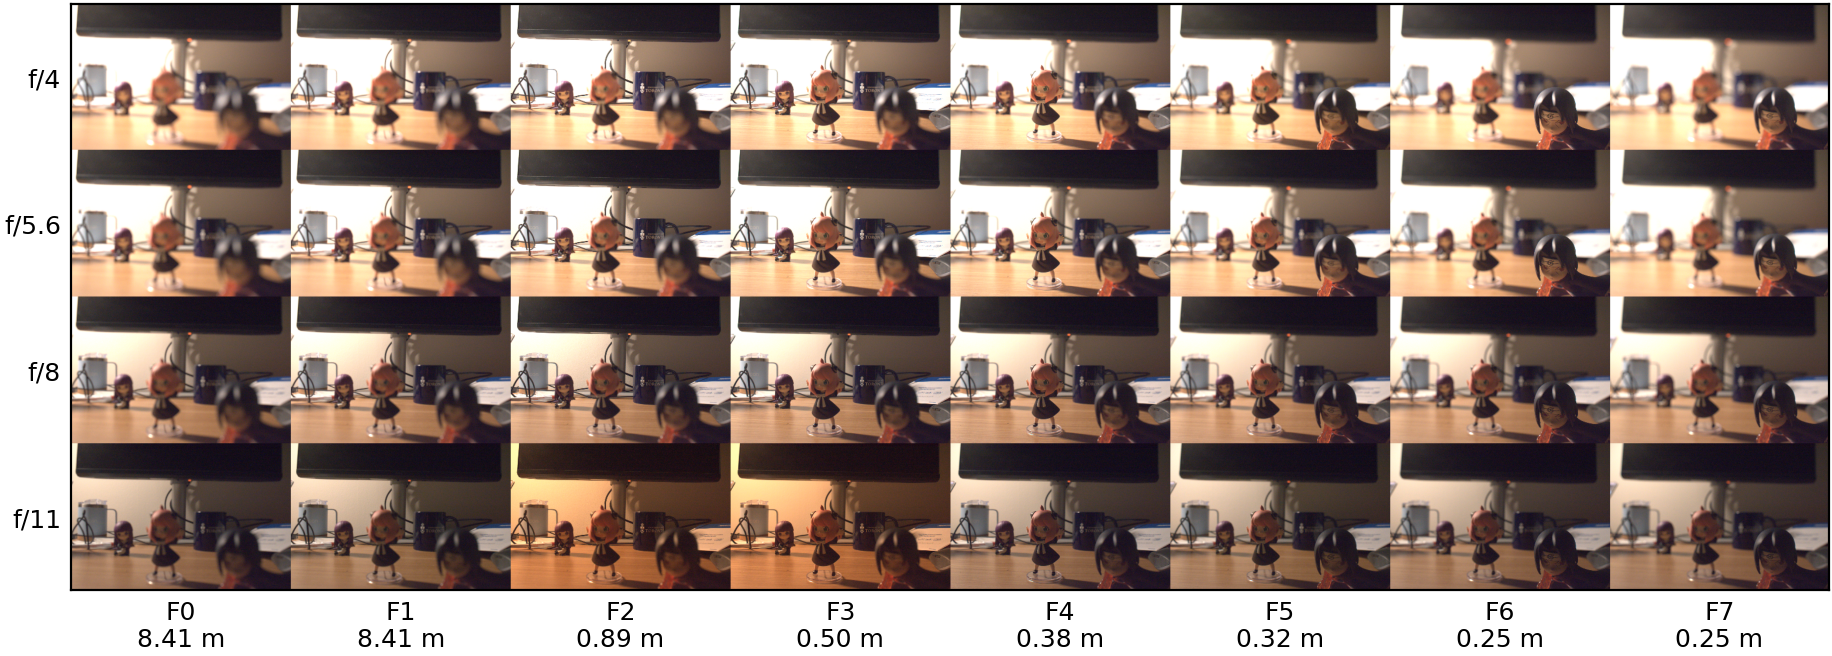
\includegraphics[width=\linewidth]{p4_stack.png}
\caption{The captured focal-aperture stack before alignment (rows: apertures; columns: focus settings with their EXIF focusing distance). All images are displayed with the same brightness gain, so the smaller apertures appear darker.}
\label{fig:p4stack}
\end{figure}
\begin{figure}[H]
\centering
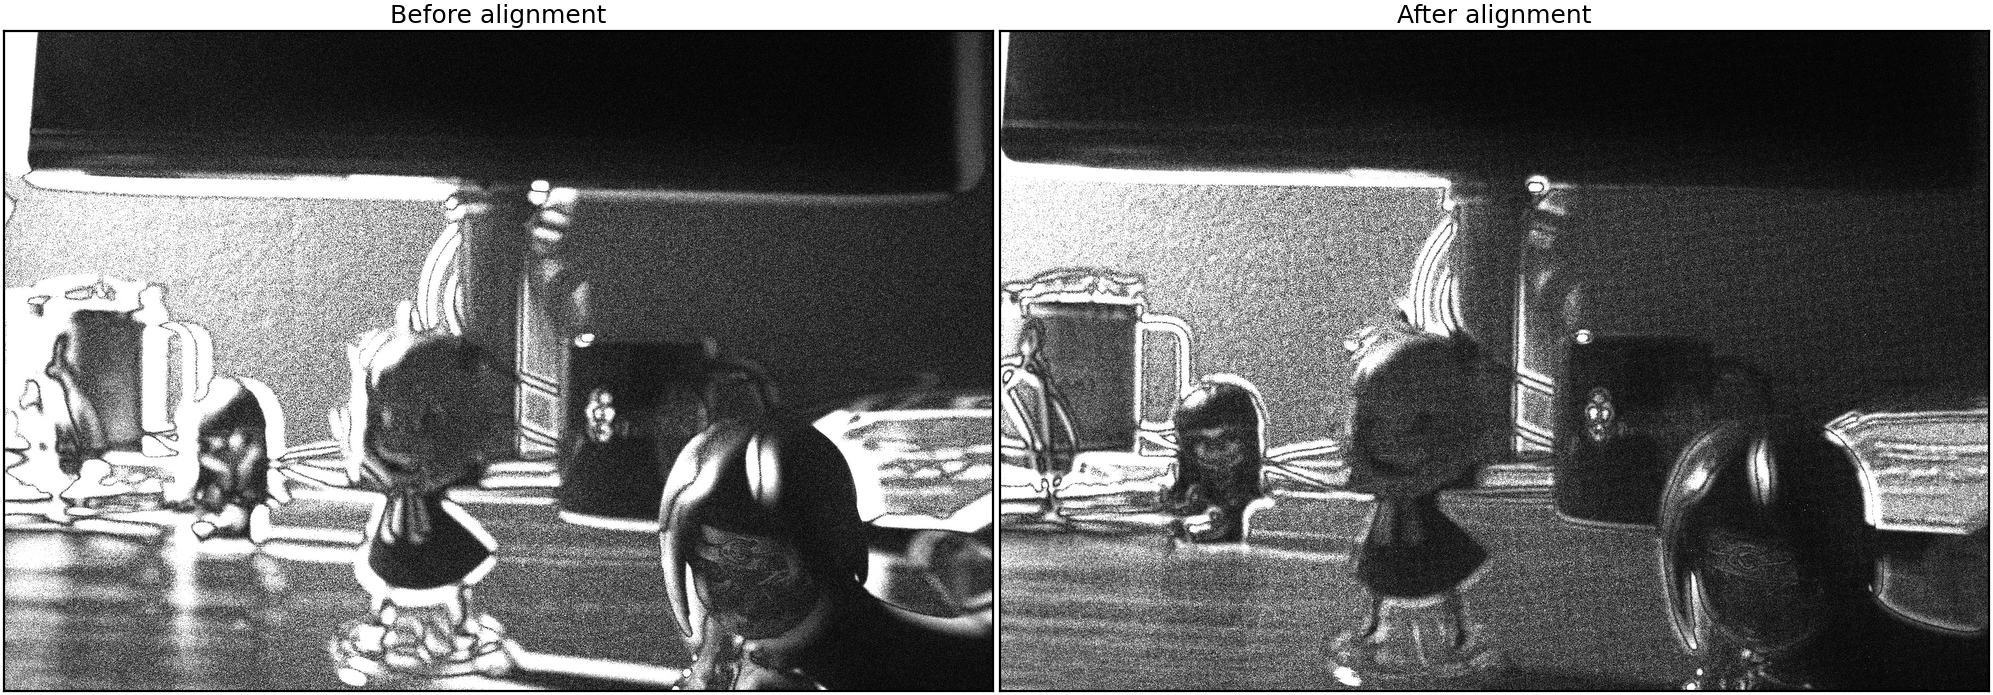
\includegraphics[width=\linewidth]{p4_alignment.png}
\caption{Absolute difference between the far-focus (F0) and near-focus (F7) images at $f/11$, before and after alignment. Before alignment, every edge is doubled by the 5\% change in magnification; after alignment, only differences due to defocus and noise remain. The bright region on the left of the first panel is caused by the change in daylight.}
\label{fig:p4align}
\end{figure}
\begin{figure}[H]
\centering
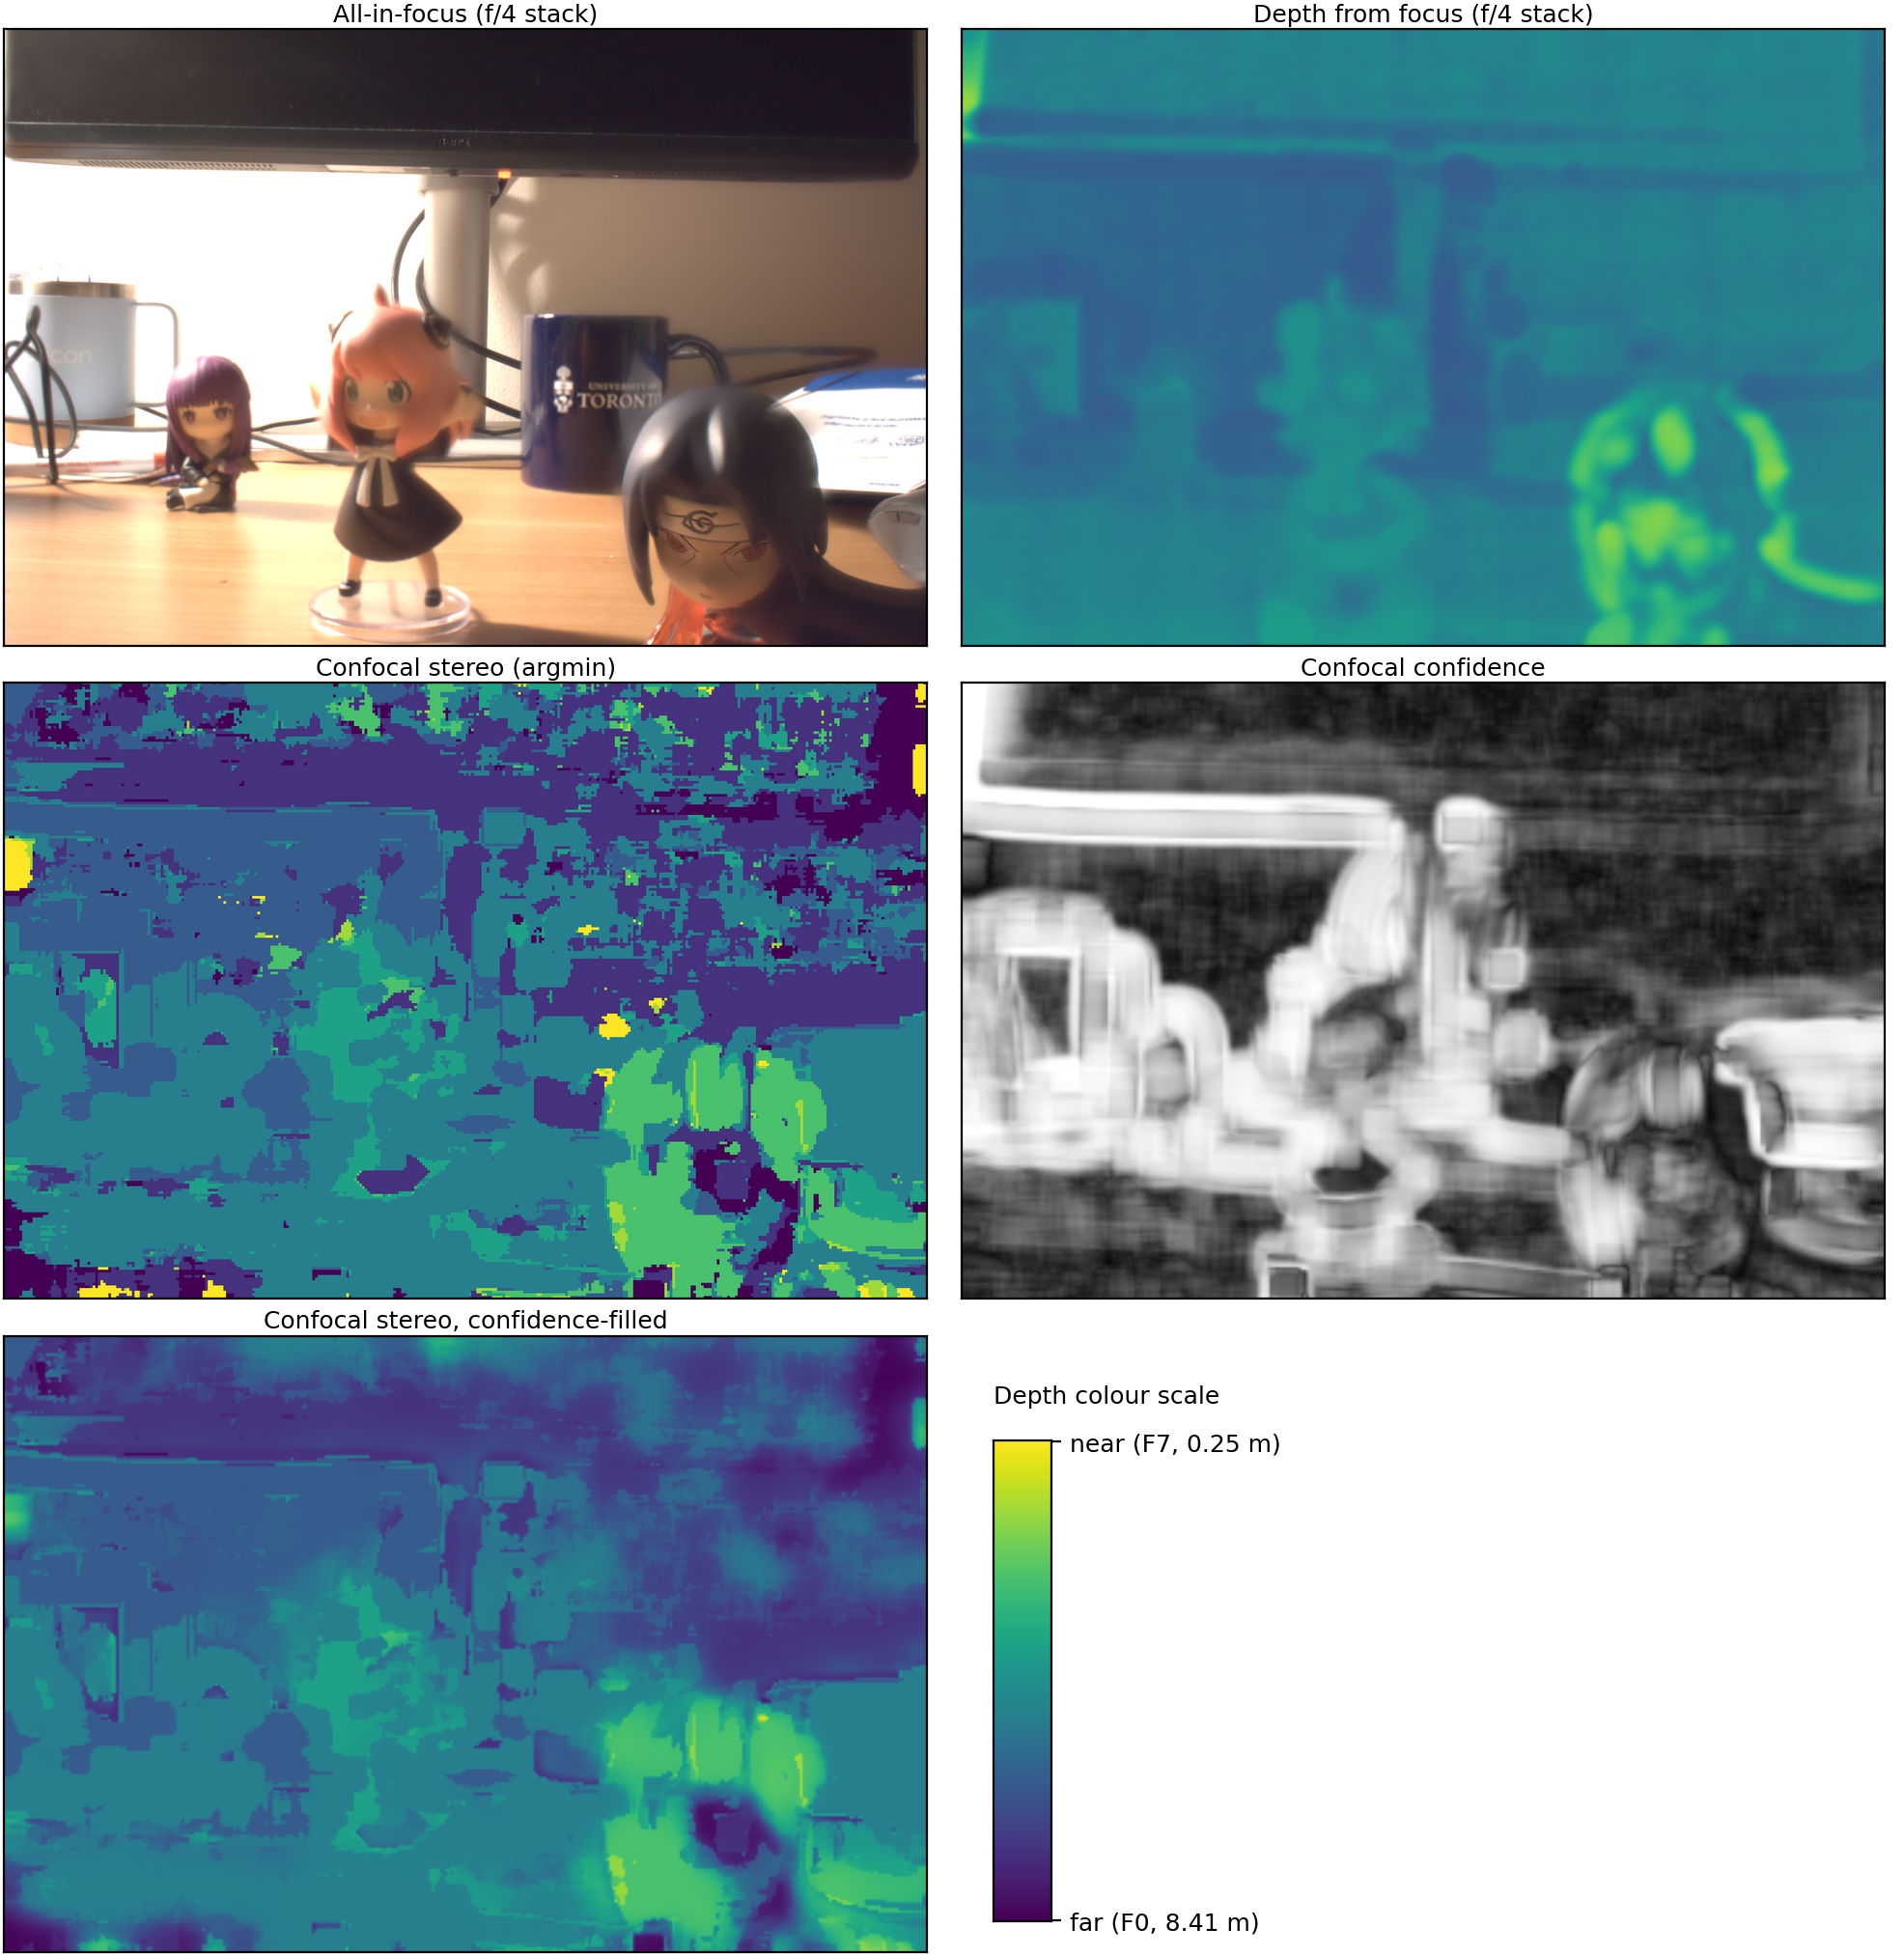
\includegraphics[width=\linewidth]{p4_results.png}
\caption{All-in-focus image and depth from focus from the $f/4$ stack, and confocal stereo from all four apertures: the per-pixel $\arg\min$, its confidence, and the confidence-filled depth map.}
\label{fig:p4results}
\end{figure}

%======================================================================
\clearpage
\section*{Acknowledgement}
The visualizations and the writing of this report were prepared in collaboration with Claude Code (Claude Opus 5.5).

\end{document}
